
\documentclass[openany,a4paper,12pt]{memoir}
%openany causes margins to be different between odd and even pages
\usepackage[left=2cm,right=2cm,top=2cm,bottom=2cm]{geometry}
%\usepackage[utf8]{inputenc}
\usepackage{graphicx}

\graphicspath{{images/}}
\usepackage{hyperref}
\usepackage[table,xcdraw]{xcolor}

\usepackage{fontspec}
%Set custom font, requires  XeLatex
\setmainfont[Ligatures=TeX]{Arial}

%Remove chapter numbering
\usepackage[pagestyles]{titlesec}
\titlespacing*{\chapter}{0pt}{*0}{12pt}
\titlespacing*{\section}{0pt}{*-2}{10pt}
\titlespacing*{\subsection}{0pt}{*-2}{10pt}
\titleformat{\chapter}[display]{\normalfont\bfseries}{}{0pt}{\Huge}
\titleformat{\section}[display]{\normalfont\bfseries}{}{0pt}{\Large}
\titleformat{\subsection}[display]{\normalfont\bfseries}{}{0pt}{\normalsize}
\newpagestyle{mystyle}
{\sethead[\thepage][][\chaptertitle]{}{}{\thepage}}
\pagestyle{mystyle}
\setlength\parindent{0pt}
\setlength{\parskip}{0.2em}

\newcommand{\screenshot}[1]{\begin{figure}[h]
    %\centering
    \fbox{\includegraphics[scale=.40]{#1}}
\end{figure}}

\newcommand{\encodersimpl}[4]{
    \multicolumn{2}{|l|}{\cellcolor[HTML]{C0C0C0}\textbf{Encoder Assignment \hspace{8.3cm} }}  \\[3pt] \hline
    Encoder 1                          & #1                         \\[3pt]  \hline
    Encoder 2                          & #2                         \\[3pt]  \hline
    Encoder 3                          & #3                         \\[3pt]  \hline
    Encoder 4                          & #4                         \\[3pt]  \hline
%\begin{itemize}
%	\item \textbf{[ Encoder 1 ]: } #1
%	\item \textbf{[ Encoder 2 ]: } #2
%	\item \textbf{[ Encoder 3 ]: } #3
%	\item \textbf{[ Encoder 4 ]: } #4
%\end{itemize}
}

\newcommand{\buttonsimpl}[4]{
    \multicolumn{2}{|l|}{\cellcolor[HTML]{C0C0C0}\textbf{Function Button Assignment \hspace{6.7cm} }}  \\[3pt] \hline
    Save | No                          & #1                         \\[3pt]  \hline
    Page                               & #2                         \\[3pt]  \hline
    Load | Yes                         & #3                         \\[3pt]  \hline
    Shift                              & #4                         \\[3pt]  \hline
}

\newcommand{\encoders}[4]{
\begin{figure}[h]
    %\centering
    \begin{tabular}{|
    >{\columncolor[HTML]{C0C0C0}}l |l|}
    \hline
    \encodersimpl{#1}{#2}{#3}{#4}
    \end{tabular}
\end{figure}
}

\newcommand{\buttons}[4]{
\begin{figure}[h]
    %\centering
    \begin{tabular}{|
    >{\columncolor[HTML]{C0C0C0}}l |l|}
    \hline
    \buttonsimpl{#1}{#2}{#3}{#4}
    \end{tabular}
\end{figure}
}

\newcommand{\encodersbuttons}[8]{
\begin{figure}[h]
    %\centering
    \begin{tabular}{|
    >{\columncolor[HTML]{C0C0C0}}l |l|}
    \hline
    \encodersimpl{#1}{#2}{#3}{#4}
    \buttonsimpl{#5}{#6}{#7}{#8}
    \end{tabular}
\end{figure}
}
\setlength\cftsectionnumwidth{3em}
\begin{document}
\author{
    Justin Mammarella
    \and
    Yatao Li
}
\title{MegaCommand Live}
\date{July 2021}

\frontmatter

	\begin{center}
	%\vspace*{\fill}
	\vspace*{5.75cm}
	\includegraphics{mcl_logo_black_short.png}
    \vspace*{1.00cm}
	\LARGE
	\vspace*{0.65cm}
	\\MegaCommand Live
    \large
	\\Firmware Version 4.00
	\footnote{Manual Revision: 22/08/2021}
    \vspace*{2cm}
    \\Justin Mammarella
    \\Yatao Li
\end{center}

\newpage
Thankyou to the community of builders, creators\\
and users that have emerged and contributed\\
their time and enthusiasm to our project.\\\\
A special mention to the testing team who have\\
helped us reflect and improve:\\\\
Waftlord\\
Moritz\\
Dataline\\
%\maketitle
\mainmatter
\tableofcontents


\chapter{Introduction}
\section{Preface}
\begin{small}
\textbf{\textit{The following document is intended to be read as a user manual for the MegaCommand Live OS. To learn how to build a DIY MegaCommand MIDI controller please see the link below \footnote{DIY MegaCommand hardware documentation: \url{https://github.com/jmamma/MegaCommand_Design}.}.}}

\end{small}

\section{Hello}
MegaCommand Live (MCL) is a firmware designed for the MegaCommand (MC) MIDI controller that expands the Elektron Machinedrum's (MD) sequencing, sound design and live performance capabilities. 
\\
\\
MCL is developed alongside the Machinedrum X OS. Together they create the modern sequencer enhancement for the Elektron Machinedrum. The MD provides the GUI and synthesis components, whilst the sequencing is now performed within the MegaCommand.
\\
\\
The MC's sequencer consists of 22 tracks each with individual length, parameter locks, micro-timing, conditional trigs, slides, mutes and an arpeggiator. Sixteen of these tracks are dedicated to the MD, the remaining six tracks are polyphonic and can be used to drive an additional MIDI device.
\\
\\
Projects are stored on the MC's SD Card. Each project utilises a grid and slot system to save and load tracks. Unlike the MD, tracks are not bound to a specific pattern or Kit, but instead can be loaded freely between different rows (patterns). Track loading can be automated and slots chained together to create dynamic musical phrases or songs. 
\\
\\
Other features of the MCL firmware include: Chromatic + Polyphonic Mode,  Level Mixer, Performance Controllers, Audio Mute + Routing System,  Sample + Sound Management, Single Cycle Waveform Designer, Global LFO, FX Pages, Automated RAM recording, USB MIDI, and much more.
\\
\\
A great deal of care has gone in to this project. Both MCL and MDX have been optimised to provide outstanding MIDI and sequencing performance, at TURBO speeds.
\\
\\
We have intended to make the firmware as intuitive as possible, particularly for users already familiar with the MD. Please take your time to read each section of this manual carefully. 
\\
\\
Let's get started.
\chapter{MegaCommand Hardware}
The MegaCommand is an Open Source MIDI controller developed to run the MCL OS. It is currently available in two form factors, the MegaCommand DIY (2017) and the MegaCMD (2021). Both were designed by Justin Mammarella.\\\\
The MegaCommand DIY is built upon the Arduino Mega 2560 development board; requiring skills in both soldering and self assembly. The MegaCMD is a pre-built version based on a new SMD design, requiring no user assembly.\\\\
The MegaCMD benefits from some additional circuitry that allows USB disk access to the MicroSD card for file transfer between a host computer.\\\\
The MegaCommand can be powered via a standard DC power jack whilst the MegaCMD only accepts power via USB.
\\\\
The MiniCommand (2010) is an older controller developed by Ruin \& Wesen that paved the development of the MegaCommand, it is not compatible with the current version of MCL.
\chapter{Terminology and Conventions}
   \begin{itemize}
      \item MCL - MegaCommand Live OS.
      \item MD - Machinedrum
      \item MDX - Machinedrum X OS.
      \item MC - MegaCommand or MegaCMD MIDI controller
      \item \textbf{<Button> } Enclosed arrows will reference the use of a MegaCommand function button to perform an action.
      \item \textbf{[Key] } Enclosed square brackets will reference the use of a Machinedrum key to perform an action. 
   \end{itemize}


\newpage
\chapter{Key Concepts}

\begin{itemize}
\item \textbf{Page:}
\\
The MCL firmware consists of pages accessible through either the MC's or MD's GUI. Each page contains distinct functionality and is described in this manual.
\item \textbf{Project:}
\\
A project stored on the Micro SD-Card.
The maximum number of projects is only limited by the SD Card capacity.

\item \textbf{Grid:}
\\
The MCL Firmware uses a Grid \& Slot system to store Tracks.\\
Each project contains two grids, X and Y. Grid dimensions are 16 Slots x 128 Rows.\\
\\
Grid X is used to store 16 MD tracks.\\Grid Y is used to store 6 External MIDI tracks + 4 AUX tracks.
\item \textbf{Bank:}\\
The rows of the Grid X are divided in to groups of 16, forming 8 banks A,B,C,D,E,F,G,H.
\item \textbf{Row/Pattern:}
\\
A row of the Grid.

\item \textbf{Slot:}
\\
A position in the Grid where a Track can be stored. (Either occupied or unoccupied).
\item \textbf{Track:}
\\
An MCL sequencer track that may contain both sound and MIDI sequencer data.

There are 3 types of tracks.
\begin{itemize}

\item \textbf{MachineDrum Track} (Grid X: Slots 1-16):
A sequencer track for the Elektron MD. Each MD Track contains the Machine's Sound Settings and Sequencer Data.

\item \textbf{External MIDI Track} (Grid Y: Slots 1-6):
A polyphonic sequencer track used to control a sound module connected via MIDI. Each External MIDI track contains Sequencer Data, and for supported Elektron devices sound data is retained. 

\item \textbf{AUX Track} (Grid Y: Slots: 13-16)\\
An auxiliary track. Used to store/recall the Machinedrum's master FX settings, LFO settings, audio Routing and Tempo settings.
\end{itemize}

\item \textbf{Device:}\\
An attached MIDI device. The MC supports a unique device on ports 1 and 2.

\item \textbf{Group:}
\\
A collection of slots ordered by the same device type.

\end{itemize}
\chapter{MIDI Setup}
\section{Connectivity:}
\textbf{Machinedrum:}
\begin{itemize}
    \item Connect the MIDI-Out of the Machinedrum to the MIDI-In (1) of the MegaCommand.
    \item Connect the MIDI-Out (1) of the MegaCommand to MIDI-In of the Machinedrum.
\end{itemize}

\textbf{Elektron Device (Analog4/MNM) (Optional):}
\begin{itemize}
    \item Connect the MIDI-Out of the Elektron to the MIDI-In (2) of the MegaCommand. 
    \item Connect the MIDI-Out (2) of the MegaCommand to MIDI-In of the Elektron.
\end{itemize}
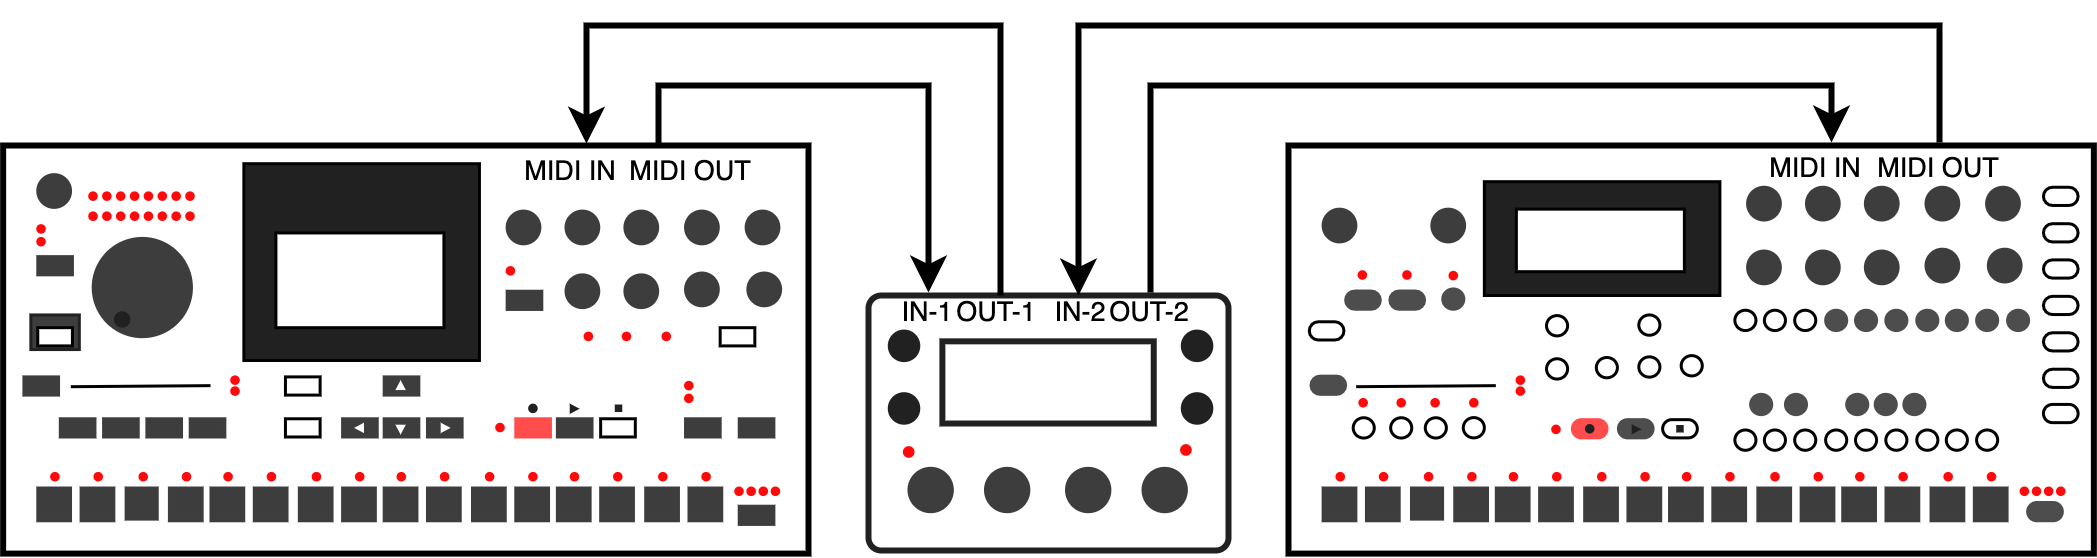
\includegraphics[width=16.55cm]{midi_machines.png}\\
\\
\textbf{External Clock (Optional):} 

\begin{itemize}
    \item A MIDI Keyboard, or sequencer can be connected to MIDI-In (2). 
    \item Attached sequencers can be used as external clock source.
\end{itemize}

\textbf{External MIDI (Optional):}

\begin{itemize}
    \item A MIDI Keyboard connected to MIDI-In (2). 
    \item MIDI-Out (2) connected to synth a module's MIDI-In.
    \item Attached MIDI Keyboards may be used to play notes in chromatic modes or via the PianoRoll editor.
    \item External synth can be sequenced from the External Sequencer Tracks.
\end{itemize}



\newpage

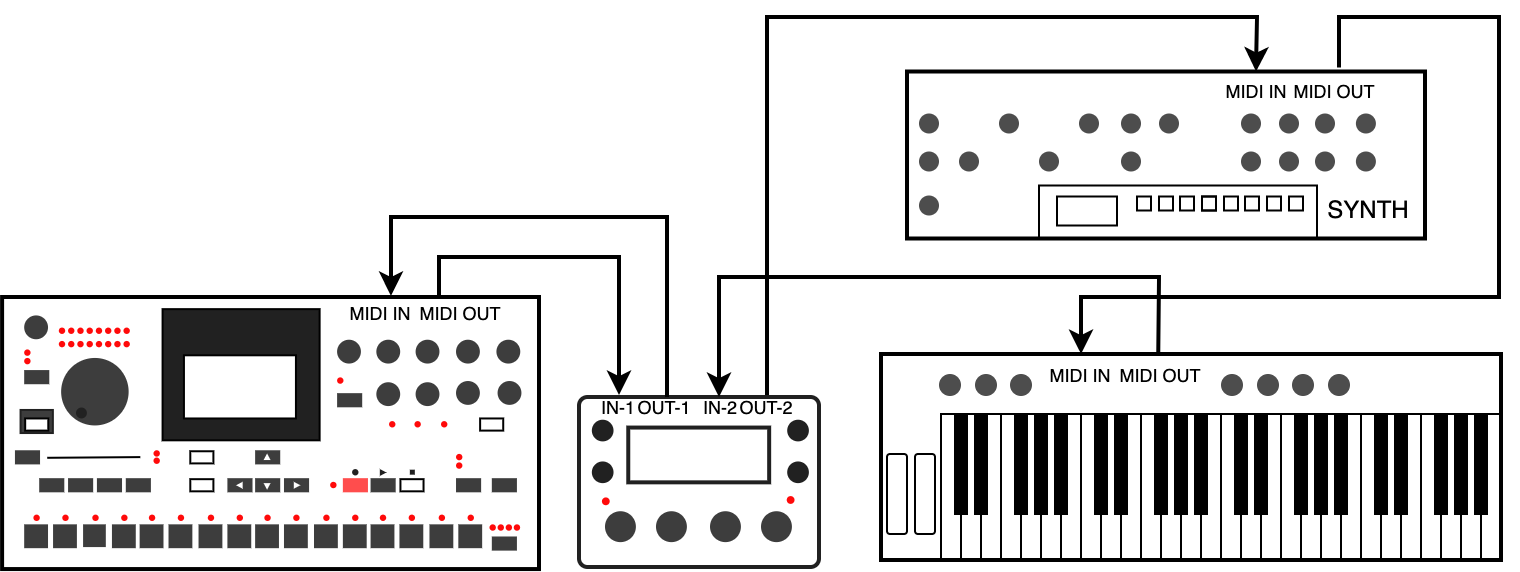
\includegraphics[width=18cm]{midi_machines2.png}\\
\section{MachineDrum Settings:}

MCL communicates with the MachineDrum using SYSEX messages, and will configure your MD's current global settings automatically.
\\\\The Machinedrum's base channel can be chosen from the MD's Global memu.

\section{Analog4 Settings:}

The following configuration must be manually applied in the Analog 4's Global Settings menu:

\begin{itemize}

\item{MIDI Port Config:}
\begin{enumerate}
\item{Output to MIDI}
\item{Input to MIDI}
\item{Keyboard CFG = EXT}
\item{Receive Notes = True}
\item{Receive CC/NPRN = True}
\end{enumerate}
\item{MIDI Channels:}

Tracks 1-6 channels need to be set to MIDI Channels 1-6 respectively.

\end{itemize}

\chapter{GUI}
\begin{center}
   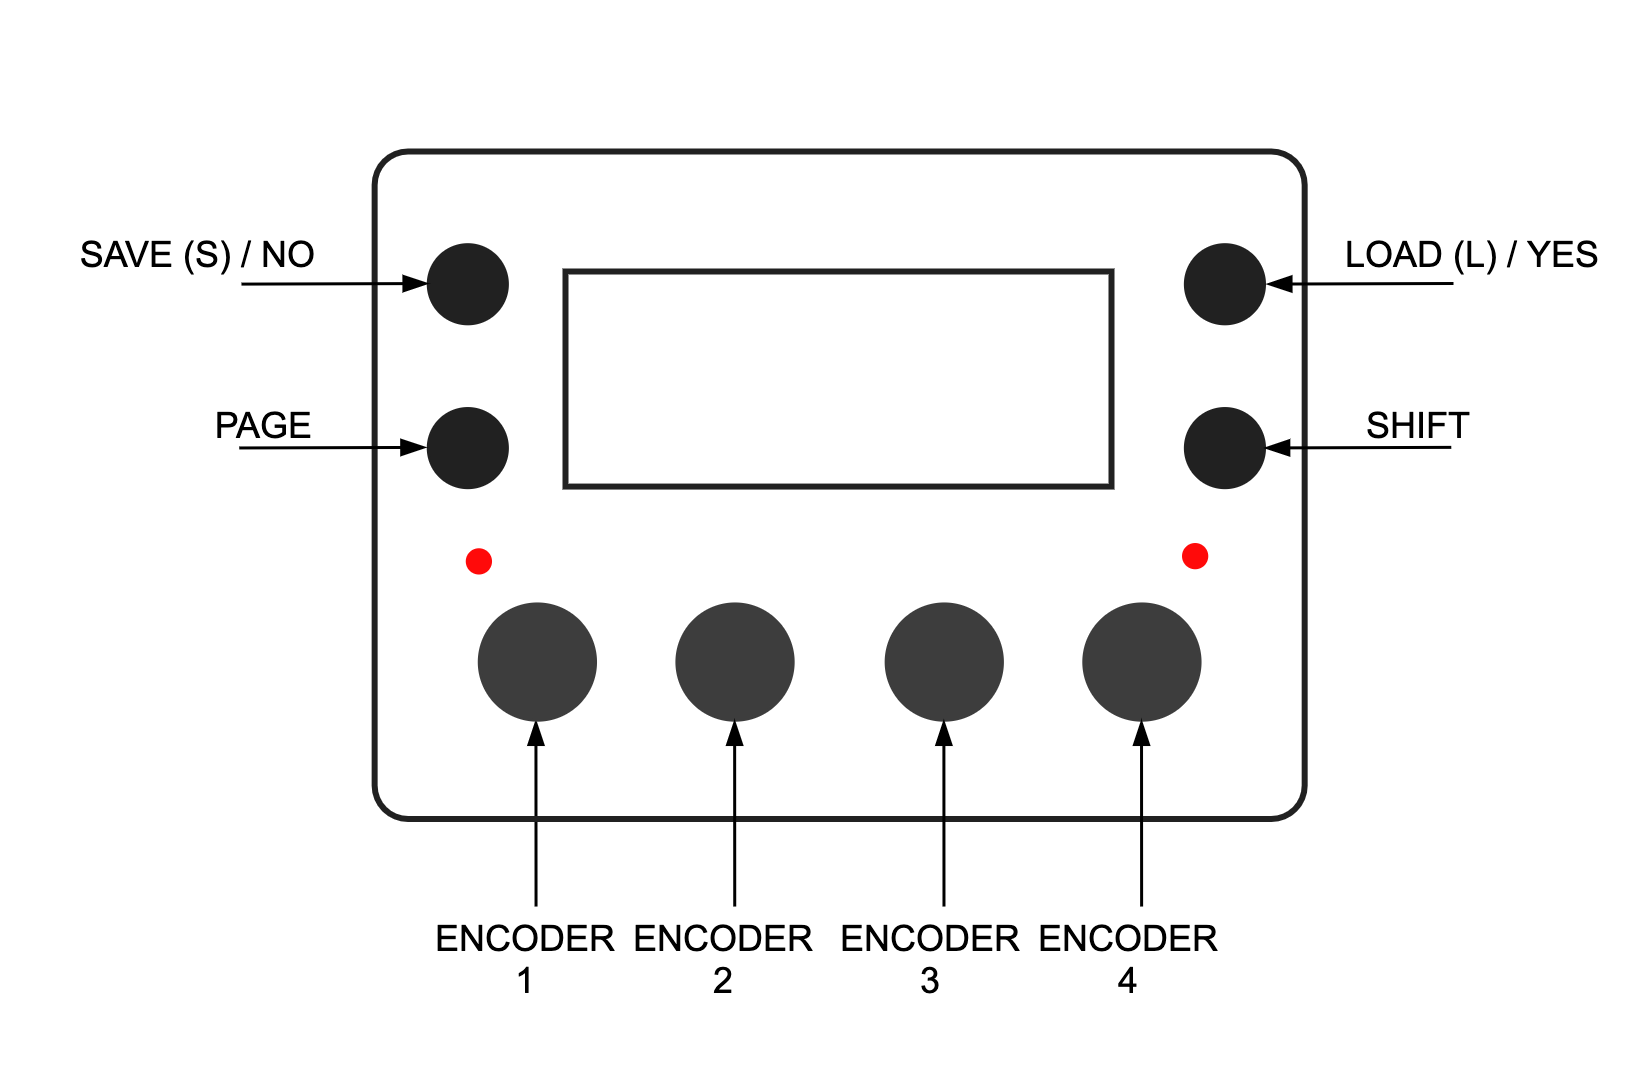
\includegraphics[width=18cm]{megacommand_gui.png}
\end{center}
\section{Function Buttons:}
From the Grid Page the function buttons perform the following actions:
\begin{itemize}
\item{\textbf{<Save | No>}: Enters the Save Page.}
\item{\textbf{<Load | Yes>}: Enters the Load page.}
\item{\textbf{<Page>}: Enters the PageSelect page.}
\item{\textbf{<Shift | Menu>}: Opens the slot Menu. }
\end{itemize}
Combined Button Presses:
\begin{itemize}
\item{\textbf{<Save | No> + <Load | Yes>}: Opens the MCL Configuration menu. }
\end{itemize}

\section{Encoder Buttons}
Encoder buttons are used to increase the speed of parameter rotation.
Holding down an encoder button whilst rotating the encoder will increase the update speed by 4x.

\newpage
\section{Machinedrum GUI: Enhanced Mode}
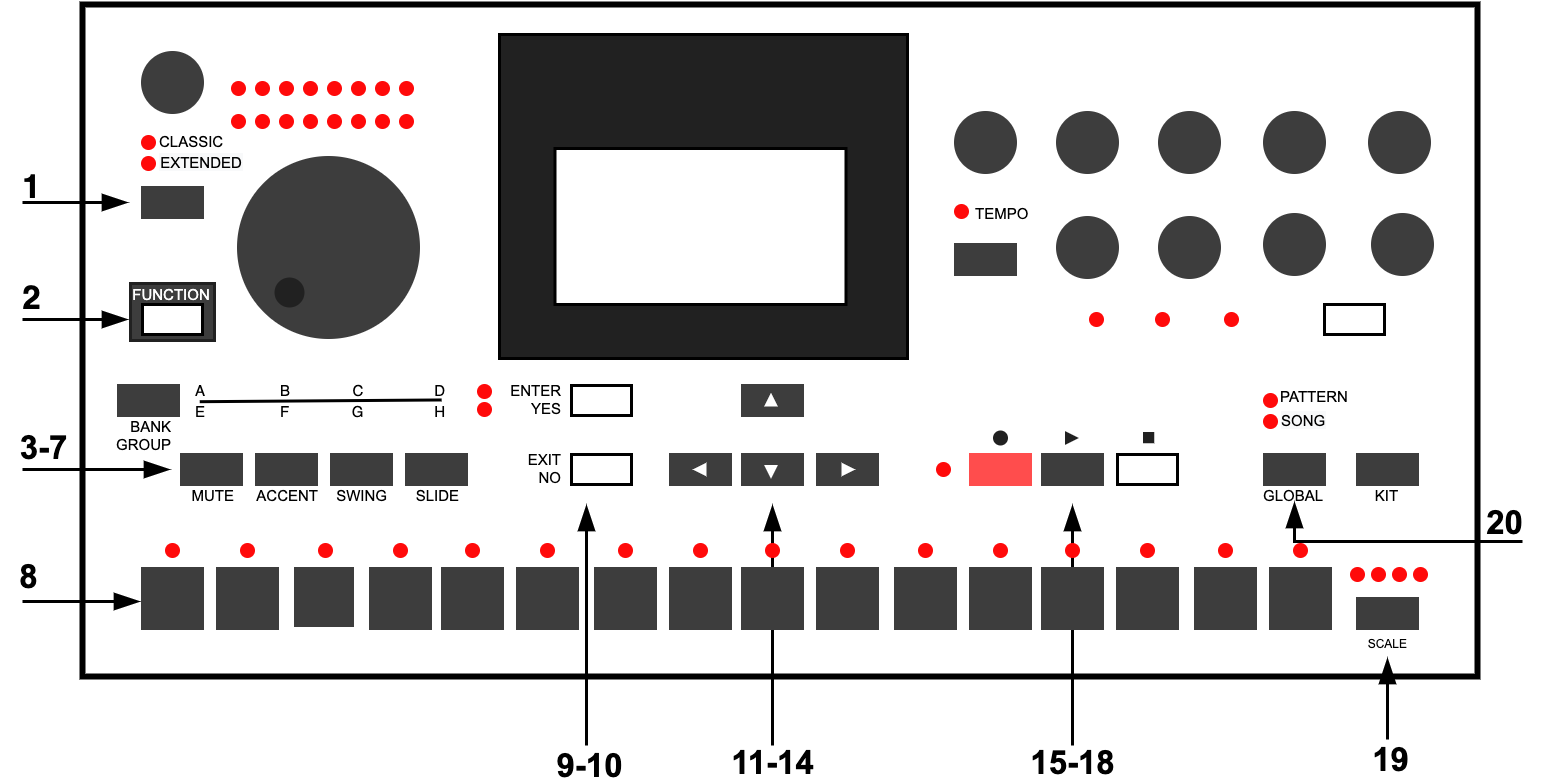
\includegraphics[width=18cm]{machinedrum_gui.png}

Version X.05 of the MD firmware introduces a third editing mode beyond Classic and Extended named \textbf{Enhanced Mode}.\\
\\
Enhanced mode is activated automatically when the MD is connected to the MegaCommand.\\
\\
When in Enhanced mode, both Classic and Extended LEDs will be lit. The three modes can be toggled using the Classic/Extended button.\\
\\
Enhanced mode enables the Machinedrum's GUI to be fully integrated with MCL as described on the next page.
\\
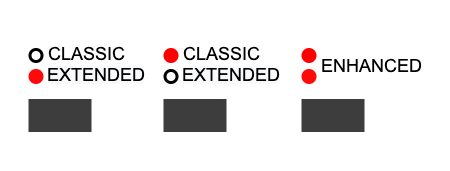
\includegraphics[width=10cm]{enhanced_mode.png}
\newpage
\section{MD + MCL command summary}
\begin{itemize}
\item \textbf{General:}
   \begin{itemize}
      \item \textbf{[Classic/Extended] } toggle between Classic, Extended and Enhanced Modes.
      \item \textbf{[Global] + [Trig] } page select.
      \item \textbf{[Bank] + [Trig]} loads slots from the selected row according to group selection.
      \item \textbf{[Bank] + [Multiple Trigs]} creates a chain of slots from selected rows according to group selection.
   \end{itemize}

\item \textbf{Grid Page:}
    \begin{itemize}
      \item \textbf{[Up/Down/Left/Right]} move grid cursor.
      \item \textbf{[Bank]} move grid cursor to start of bank.
      \item \textbf{[Clear/Copy/Paste]} all MD tracks.
      \item \textbf{[Function] + [Scale]} Pattern length and speed settings can be set via the MD's scale menu.
      \item Hold \textbf{[No]} key to open Slot Menu.
      \begin{itemize}
                \item \textbf{[Bank]} keys can be used to select load mode: Manual, Auto or Queue.
                \item \textbf{[Up/Down/Left/Right]} to select multiple slots in the grid.
                \item \textbf{[Clear/Copy/Paste]} to clear/copy/paste selected slot(s).
                \item \textbf{[Yes]} load selected slots. Slots are loaded according to the load mode. If more than one row is selected, slots in the same column will be automatically chained.
      \end{itemize}

\item \textbf{[Yes]} opens \textbf{Load Page:}
    \begin{itemize}
    \item Hold \textbf{[Yes]} to open slot Group Select. Release \textbf{[Yes]} to load groups. Groups selection editable via \textbf{[Trig]} keys 1-4.
    \item \textbf{[Trig]} keys are used to select and load sequencer tracks from slots of the current row.
    \item \textbf{[Bank]} keys can be used to quickly select the load mode: Manual, Auto or Queue.
    \end{itemize}
    
\item \textbf{[Func] + [Yes]} opens \textbf{Save Page:}
    \begin{itemize}
    \item Hold \textbf{[Yes]} to open slot Group Select. Release \textbf{[Yes]} to save groups.  Groups selection editable via \textbf{[Trig]} keys 1-4.
    \item \textbf{[Trig]} keys are used to select and save sequencer tracks to slots of the current row.
    \item \textbf{[Bank]} keys can be used to quickly select the save mode: Save, Merge or Import.
    \end{itemize}
\end{itemize}

\item \textbf{Mixer Page:}
      \begin{itemize}
       \item \textbf{[Trigs] + [MD Encoder]} simultaneously modify parameters across selected tracks. 
      \item \textbf{[No] + [Trig]} revert parameter for selected track.
       \end{itemize}

\item \textbf{Chromatic Page:}
      \begin{itemize}
      \item \textbf{[Up/Down]} change octave
      \item \textbf{[Left/Right]} transpose
      \end{itemize}

\item \textbf{Sequencer:}
\begin{itemize}
      \item \textbf{[Record]} key to enter/exit step editing.
      \item \textbf{[Record] + [Play]} to enter realtime record mode (on any page).
      \item \textbf{[Clear/Copy/Paste]} Clear/Copy/Paste for Track/Page/Step.
      \item \textbf{[Step] + [Left/Right]} Microtiming.
      \item \textbf{[Step] + [Up/Down]} Conditional.
      \item \textbf{[Function] + [Left/Right]} Shift track.
      \item \textbf{[Function] + [Up]} Reverse track.
      \item \textbf{[Function] + [Scale]} Track length and speed settings can be set via the MD's scale menu.
      \item \textbf{[Function] + [Bank B]} Edit Lock toggle
      \item \textbf{[Function] + [Bank C]} Edit Mute toggle
      \item \textbf{[Function] + [Bank D]} Edit Slide toggle
\end{itemize}
\end{itemize}




\chapter{Page Select Menu}
The PageSelect menu is accessed by holding the MD's \textbf{[Bank Group]} key.
\screenshot{page_select_page.png}

The PageSelect menu allows quick navigation between MCL pages.
\\
\\
When open, the PageSelect menu displays the Page to be loaded. The MD's \textbf{[Trig]} keys can be used to quickly toggle between pages in the PageSelect menu, releasing the MD's \textbf{[Bank Group]} key will load the selected page.
\\
\\
The pages are grouped into four categories. The category of the current selected page is highlighted on the display:

\begin{figure}[h]
    \begin{tabular}{|l|l|l|l|}
    \hline
    \rowcolor[HTML]{C0C0C0} 
    1    & 2              & 3          & 4              \\ \hline
    MAIN & SEQ(Sequencer) & SND(Sound) & AUX(Auxiliary) \\ \hline
    \end{tabular}
\end{figure}
\textit{ The page numbers below correspond to their mapping over the \textbf{[Trig]} keys. }


\begin{figure}[h]
    \begin{tabular}{|l|l|l|l|l|}
    \hline
    \rowcolor[HTML]{C0C0C0} 
    {\color[HTML]{000000} Group} & \multicolumn{4}{l|}{\cellcolor[HTML]{C0C0C0}{\color[HTML]{000000} Pages}}      \\ \hline
    MAIN                              & 1. Grid            & 2. Mixer         & 3. Perf           & 4. Route            \\ \hline
    SEQ                               & 5. Step Editor & 6. LFO & 7. PianoRoll Editor & 8. Chromatic Mode \\ \hline
    SND                               & 9. Sound Manager   & 10. WAV Designer & 11. --       & 12. --      \\ \hline
    AUX                               & 13. FX Delay       & 14. FX Reverb    & 15. RAM 1          & 16. RAM 2         \\ \hline
    \end{tabular}
\end{figure}









\chapter{Configuration Menu}
The Configuration Menu is used for project management and to change a variety of software and hardware settings.

\screenshot{global_menu_1.png}
%\fbox{\includegraphics[scale=.40]{global_menu_1.png}}\\\\
%\fbox{\includegraphics[scale=.40]{global_menu_2.png}}\\

\textit{The Configuration menu can be opened via the GridPage by pressing the \textbf{<Save> and <Load>} buttons simultaneously.}\\\\
To enter sub-menus press the \textbf{<YES>} button. Press the \textbf{<NO>} button to go back one level or exit the menu.
\section{Load Project:}
The Load Project sub-menu will display a list of MCL Projects that are stored on the root folder of the Micro SD card.\\\\
The current project is always selected first and is indicated by an '>' character next to its name.
\screenshot{project_menu.png}
%\fbox{
\includegraphics[scale=.40]{project_menu.png}}\\

\subsection{Delete or Rename Project:}
From the file options menu, you can delete or rename projects.\\\\
\textit{From within the Load Project page, press and hold \textbf{<Shift>} to access the file options menu.\\
Use the encoder to make your selection, release \textbf{<Shift>} to activate your choice.}

\newpage
\section{New Project:}
The New Project options loads the New Project Page. This page allows you to specify a name for a project which will then be created.\\
%\fbox{
\includegraphics[scale=.40]{new_project.png}}\\
\screenshot{new_project.png}

\screenshot{charpane.png}
\textit{All text editing pages in MCL allow access to char pane. Hold \textbf{[ Shift1 ]}}

\section{Project Files:}
Projects are stored on the SD Card in the \textbackslash{}Projects\textbackslash{} directory.
Each project has its own folder, inside the project folder there are 3 files:
\begin{verbatim}
\Projects\new_project_000\
                          |- new_project_000.mcl   <- Project master file
                          |- new_project_000.0     <- Grid X data
                          |- new_project_000.1     <- Grid Y data
\end{verbatim}
\chapter{MIDI Settings Menu:}
The MIDI menu provides access to seven MIDI configuration sub-menus.
\screenshot{midi_menu.png}
\\
\textit{Changes made in each MIDI configuration are applied upon menu exit.}

\section{Port Config:}
The Port Config menu is used to configure the MIDI port settings.
\screenshot{midi_ports_menu.png}\\
\begin{tabular}{|l|l|}
\hline
\rowcolor[HTML]{C0C0C0} 
Entry                                  & Function                                                                       \\ \hline
TURBO 1: {[} 1x, 2x, 4x, 8x {]}        & Port 1's Turbo MIDI speed                                                             \\ \hline
TURBO 2: {[} 1x, 2x, 4x, 8x {]}        & Port 2's Turbo MIDI speed                                                             \\ \hline
TURBO USB: {[} 1x, 2x, 4x, 8x {]}      & USB Port's Turbo MIDI speed                                                           \\ \hline
Driver 2: {[} Gener, Elekt {]}         &  Port 2's MIDI driver, either Generic or Elektron                                   \\ \hline
CTRL Port: {[} 2, USB, 2 + USB) {]}    & Which MIDI port provides control input (Note + CC)\\& for Sequencer + Chromatic pages.  \\ \hline                                    
\end{tabular}
\\\\
\textit{If using the Machinedrum MK1, set Turbo Speed no greater than 4x.}\\\\
\textit{{If you are intending to pair your Megacommand with a supported Elektron device}
(MNM, A4) set \textbf{Driver 2}  to Elektron. For all other MIDI devices (including unsupported Elektron machines), set \textbf{Driver 2} to General MIDI (default setting).}\\\\
\textit{If you are intending to use the paired Elektron device's MIDI thru to control further external equipment, you must set Turbo 2 speed to 1x.}

\newpage

\section{Sync:}
The Sync Config menu is used to configure MIDI clock + transport receive and destination settings.
\screenshot{midi_sync_menu.png}\\
\begin{tabular}{|l|l|}
\hline
\rowcolor[HTML]{C0C0C0} 
Entry                                  & Function                                                                       \\ \hline
CLOCK RECV: {[}1, 2, USB{]}                & Receive MIDI Clock from port.                                                  \\ \hline
TRANS RECV: {[}1, 2, USB{]}                & Receive MIDI Transport from port.                                               \\ \hline
CLOCK SEND: {[}OFF, 2, 2 + USB{]}          & Forward MIDI Clock to selected port(s)                                            \\ \hline
TRANS SEND: {[}OFF, 2, 2 + USB{]}          & Forward MIDI Transport to selected port(s)                                        \\ \hline
\end{tabular}
\\\\
\textit{Note: MCL does not generate its own MIDI Clock, instead it relies on a clock signal from either Port 1, Port 2 or USB.}
\\
\textit{The MD's internal clock settings are controlled by MCL and will be automatically configured based on the options selected above.}

\section{Routing:}
The MIDI Routing configuration menu can be used to set MIDI traffic forwarding between ports.
\screenshot{midi_route_menu.png}\\
\begin{tabular}{|l|l|}
\hline
\rowcolor[HTML]{C0C0C0} 
Entry                                  & Function                                                                       \\ \hline
MIDI1 FWD: {[}OFF, 2, USB, 2 + USB{]}                & Forward non-realtime MIDI data from Port 1 input \\ & to the selected MIDI output port(s).                                                \\ \hline
MIDI2 FWD: {[}OFF, 1, USB, 1 + USB{]}                & Forward non-realtime MIDI data from Port 2 input \\ & to the selected MIDI output port(s).                                               \\ \hline
USB FWD: {[}OFF, 1, 2, 1 + 2{]}          & Forward non-realtime MIDI data from USB-MIDI \\ & input to the selected MIDI output port(s).                                            \\ \hline
CC LOOP: {[}OFF, 2->2{]}          & Loopback MIDI CC messages on same port.                                      \\ \hline
\end{tabular}


\newpage
\section{Program:}
The Program menu is used to enable the sending and receiving of MIDI Program Change messages.
\screenshot{midi_prog_menu.png}\\
\begin{tabular}{|l|l|}
\hline
\rowcolor[HTML]{C0C0C0} 
Entry                                  & Function                                                                       \\ \hline
PROG Mode: {[}BASIC, ADV{]}                & Basic or Advanced. 
\\ \hline
PRG IN: {[}--, 1 .. 16, OMNI{]}            & Program change receive channel.                                            \\ \hline
PRG OUT: {[}--, 1 .. 16{]}          & Program change transmit channel.                                          \\ \hline
\end{tabular}
\begin{itemize}
    \item{\textbf{PROG Mode:} MIDI Program Change IN has two modes of operation, BASIC or ADV (Advanced).
\begin{itemize}
    \item{ \textbf{BASIC:} Program Change Receive will "Group Load" an entire row according to Load Page mode and Group Select settings. }
    \item{  \textbf{ADV:} Program change receive will set the row for slots to be loaded from.\\\\ MIDI notes from C3 upwards on Port 2 can be used to select slots to be loaded.\\\\  In this way, you can load any slot (or multiple slots) using a combination of Program Change + MIDI note. \\\\
 If Program Change is not received before MIDI note on/off, MCL will load from the current selected GUI row.\\\\ 
 MCL cannot load instantaneously, there is a minimum 1 bar delay.}
\end{itemize}}
\item{\textbf{PRG In:}
Set the receive channel for Program Change and Note messages on Port 2.\\\\
When set to -- (default) Program Change In is disabled.}
\item{\textbf{PRG Out:}
Set the send channel for Program Change messages on Port 2, which are sent when loading slots or rows.\\\\
When set to -- (default) Program Change Out is is disabled.}
\end{itemize}

\newpage

\section{MD MIDI:}
The MD MIDI configuration menu is used to configure Machinedrum driver's MIDI settings.
\screenshot{midi_md_menu.png}\\
\begin{tabular}{|l|l|}
\hline
\rowcolor[HTML]{C0C0C0} 
Entry                                  & Function                                                                       \\ \hline
CHRO CHAN: {[}--, 1..16{]}        & MIDI Channel for MD Chromatic mode. \\ \hline
POLY CHAN: {[}--, 1..16{]}         & MIDI Channel for MD Polyphonic mode. \\ \hline
TRIG CHAN: {[}--, 1..16{]}        & MIDI Channel for MD Trig mode. \\ \hline
\end{tabular}

\begin{itemize}
\item{\textbf{CHRO CHAN:} The CHRO CHAN setting is used to control which input channel the MD should receive note data from when in Chromatic mode. When set to INT (default) the MD will be controlled by the MD's \textbf{[Trig]} keys in chromatic mode. \\\\\textit{For this setting to work correctly, CTRL PORT in PORT CONFIG must also be set to the desired port.}}

\item{\textbf{POLY CHAN:} Dedicated MIDI Channel for playing designated Polyphonic tracks chromatically.}
\item{\textbf{TRIG CHAN:} Dedicated MIDI channel for triggering MD tracks via Note On message. Useful for triggering sounds using a MIDI drum pad. Track Mapping starts from note C2. Note Velocity is mapped to volume.}
\end{itemize}

\section{General MIDI:}
The General MIDI configuration menu is used to configure the Generic MIDI driver's settings.
\screenshot{general_md_menu.png}\\
\begin{tabular}{|l|l|}
\hline
\rowcolor[HTML]{C0C0C0} 
Entry                                  & Function                                                                       \\ \hline
MUTE CC: {[} 0..127,--{]}        & CC parameter for sending/receving Ext MIDI track\\& mute state on Mixer Page. \\ 
\hline
\end{tabular}
\chapter{Machinedrum Settings Menu:}
The Machinedrum settings are used to control how the MCL firmware interacts with the MD.
\screenshot{machinedrum_menu.png}
\section{Import:}
The \textbf{IMPORT} option opens the Machinedrum Pattern Import Menu.\\ 
Multiple patterns can be imported sequentially from their starting location \textbf{SRC} on the MD to a position \textbf{DEST} on the MCL grid. The \textbf{COUNT} parameter specifies the number of patterns to be imported.
\screenshot{machinedrum_import.png}
\section{Normalize:}
When the \textbf{NORMALIZE} option is set to AUTO (default), all saved MD tracks have their LEV boosted to 127, and parameters controlling VOL (including parameter locks) are lowered
to compensate. LFOs with destination VOL are 
adjusted too.\\
\\
The resulting track loudness remains the same, but the Track LEV parameter is no longer set arbitrarily. The maximum value of LEV (127), will always be the loudest volume for each track.\\
\\
When the sequencer is running, the LEV paramater is never transmitted to the MD. This allows the performer to fade tracks in and out of a mix using the LEV parameter.\\
\\
The performer can then confidently raise the LEV of the track to 127, knowing this is the is the intended maximum loudness for the track.
\section{Poly Config:}
The \textbf{POLY CONFIG} option opens the Voice Select page and allows one or more tracks of the MD to act as voices of a polyphonic synthesizer.

\chapter{System Settings Menu:}

\section{Display:}
The display setting is used to enable the OLED display mirror. Using the provided python script\footnote{\url{https://github.com/jmamma/MCL/tree/master/python}} and a USB MIDI connection between the MC and your computer, it is possible to mirror the OLED display to your computer screen.\\
\\
\textit{Leaving this setting enabled will reduce the performance of the GUI.}


\include{./TeX_files/chain_settings}
\include{./TeX_files/system_settings}
%\chapter{ Workflow: }

The Grid is similar to the banks of the MD, but different. An active pattern is first loaded from the Grid into the Internal Sequencer and then ready for playback. 

Different tracks from different rows in the Grid can be mix-and-matched into the Internal Sequencer too.

Patterns created in the Sequencer Pages are kept in the Internal Sequencer, and thus not immediately saved to the Grid, until the MCL firmware is told so in the Save Page. 

A common gotcha is to create a pattern in the Sequencer Pages, load data from the Grid, only to find the just-created pattern gone. To avoid this, make sure to \textbf{save modified internal sequence before loading}.

\chapter{Grid Page}
The first page you will be presented with after loading or creating a new project is the Grid Page. This is the main page of MCL and is used to access the firmware's sub-pages and menus.

\begin{center}
	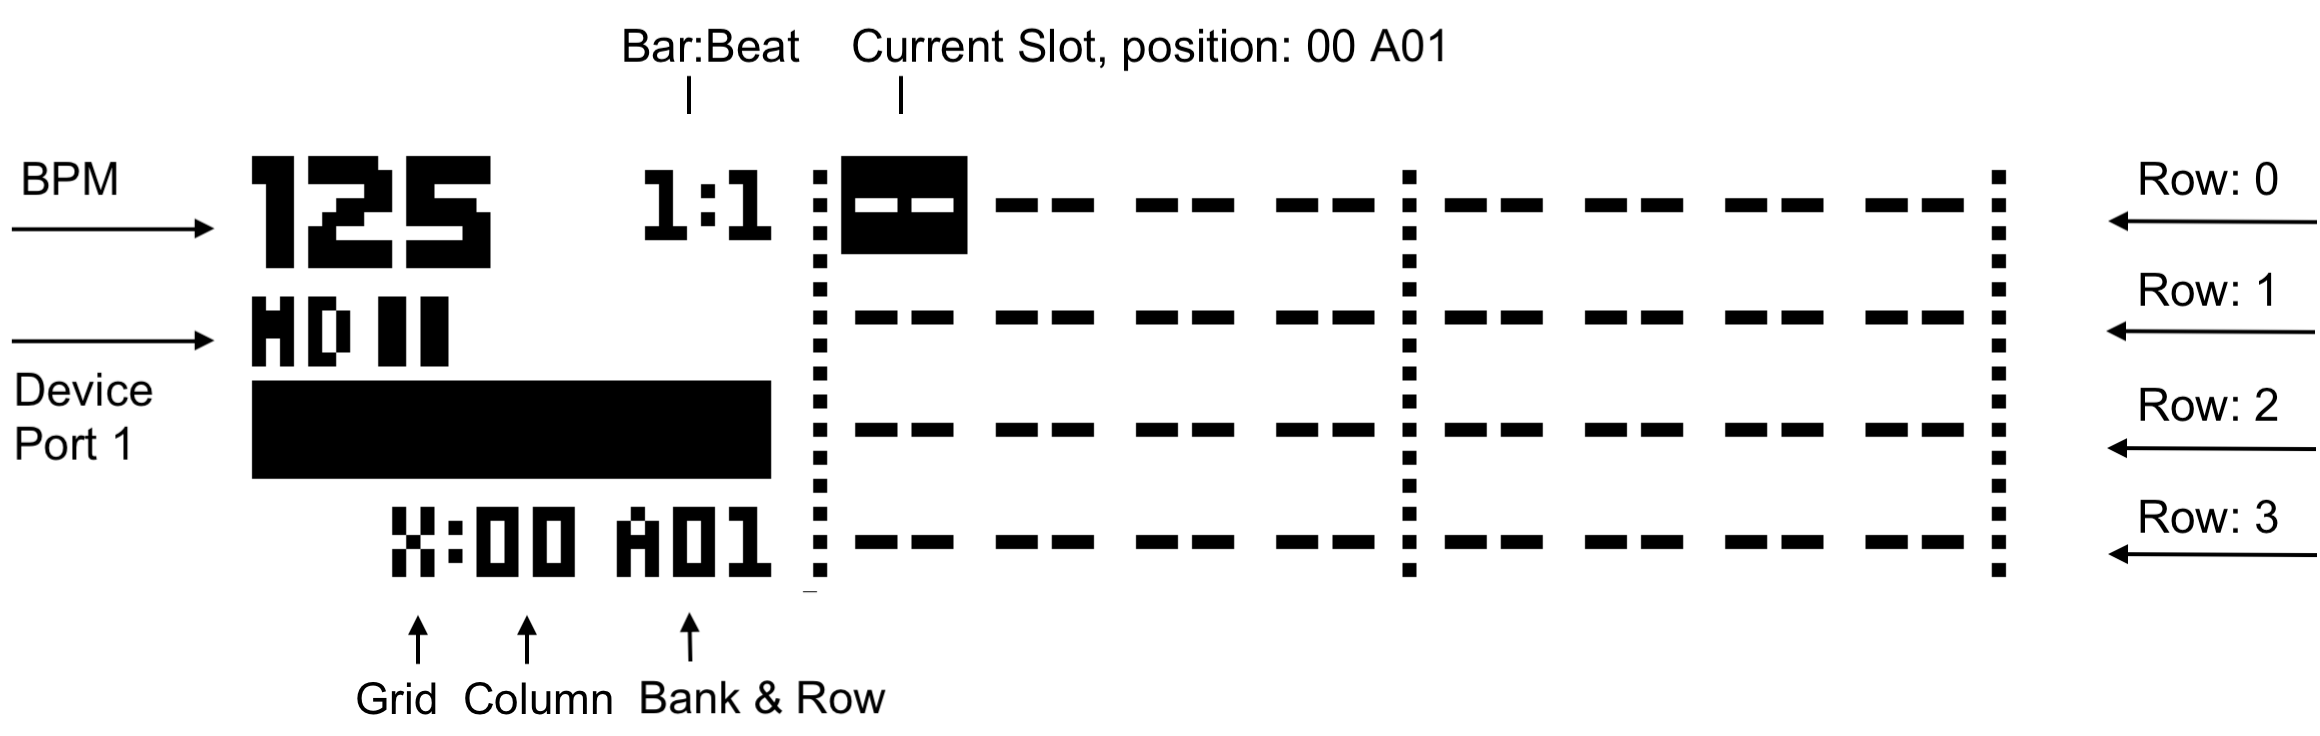
\includegraphics[scale=.40]{grid_init_annot.png}
\end{center}
MCL displays a portion of the active grid on screen. 
Eight slots across four rows are shown.\\
\\
Occupied slots will display the Machine Type associated with the track. For example "BD" for Bass Drum. Unoccupied Slots are represented by two lines of "--" . For clarity, a dashed vertical line is printed after every fourth column.\\\\
An interactive cursor indicates the current slot position and is distinguished by a slot printed with inverted colours. Rotating \textbf{<Encoder 1>} or \textbf{<Encoder 2>} will allow the cursor position to change. When the cursor reaches the edges of the screen you can continue to scroll through the grid.
\\\\
Towards the bottom left corner of the display, the active grid followed by the current slot's column and row are shown.\\\\
The active grid can be toggled between either X or Y from the Slot Menu.
\textit{When performing actions such as saving/loading they will apply to the grid that is currently active.}
\encodersbuttons{scrolls the grid horizontally.}{scrolls the grid vertically.}{--}{--}{activates Save page.}{activates PageSelect page.}{activates Load page.}{activates the Slot menu.}
\include{./TeX_files/grid_slot_system}
\chapter{Slot Menu:}

The Slot Menu is used to manipulate the properties of selected slots; to clear, copy, paste one or more slots and to configure a slot's LOOP \& JUMP settings. It also provides an option to rename the current row and to alternate the active Grid between X or Y.
\screenshot{slot_menu.png}
\\
\textit{The Slot Menu is accessible from the GridPage by holding down the \textbf{<Shift>} function button or the MD's \textbf{[No]} key.\\\\When \textbf{<Shift>} / \textbf{[No]} is released, any changes to the menu will be applied to the selected slots. }
\section{Multiple Slot Selection:}
A rectangular selection containing multiple slots can be made by entering the slot menu and rotating \textbf{< Encoder 3>} and \textbf{<Encoder 4>}. Alternatively the MD's \textbf{[Up/Down/Left/Right]} arrow keys can be used to make a selection.
\screenshot{range_copy.png}
\section{Slot loading}
When the Slot Menu is active, selected slots can be loaded by pressing the MD's \textbf{[YES]} key. 
Slots are loaded according to the current load MODE setting. If more than one row is selected, the load MODE is automatically set to QUE, and the loaded slots are added to each column's Playback Queue.
\\\\
The MD's \textbf{[Bank]} keys can be used to quickly change the load MODE setting between [ MAN, AUT, QUE ].
\\\\\
\textit{Slot loading is covered in more detail in the "Saving and Loading" section of this manual.}
\newpage
\section{Slot Menu Options:}
\begin{tabular}{|l|l|}
\hline
\rowcolor[HTML]{C0C0C0} 
Entry                                  & Function                                                                       \\ \hline
Grid: {[} X, Y {]}                     & switch between Grid X or Y.                                                      \\ \hline
Mode: {[} –, AUT, MAN, QUE {]} & \begin{tabular}[c]{@{}l@{}}AUT: sets load mode to auto. \\ MAN: sets load mode to manual.\\ QUE: sets load mode to queue.\end{tabular} \\ \hline
Len: (0, 64)                           & step length of track/slot.\\
                                           \\ \hline
Loops: (0, 64)                         & how many times to loop track/slot.\\
                                           \\ \hline
Jump: (0,127)                           & \begin{tabular}[c]{@{}l@{}}which row the current slot is to\\ load/jump to after n loops.\end{tabular}                                                                               \\ \hline

Clear: {[} –, YES {]}                  & clear the selected slot(s).                                                                                                                                                                   \\ \hline
Copy: {[} –, YES {]}                   & copy the selected slot(s).                                                                                                                                                                    \\ \hline
Paste: {[} –, YES {]}                  & paste the selected slot(s).                                            

       \\ \hline
Insert                                 & Insert a row on Grids X and Y.                                      
       \\ \hline
Rename                                 & rename the current row on Grids X and Y.                                                                                                                                                       \\ \hline
\end{tabular}
\\\\\\
\textit{The INSERT row option to the Grid Page's slot menu. Will insert N blank rows in both Grid X and Y by shifting rows beneath. Note: the Grid length is never increased and the last N rows at end of the Grid will be deleted.}
\chapter{MCL Sequencer:}
MCL features a powerful sequencer. There are 16 step sequencer tracks dedicated to the MD and 6 polyphonic tracks dedicated to External Midi devices, each has track independent length and playback speed.
\section{MD Sequencer Tracks:}
\begin{itemize}
\item 16 Track Sequencer with 64 max steps per track.
\item Conditional Trigs, Slide, Mute and Micro Timing per step.
\item 8 lockable parameters per track with 256 locks available per track.
\item Trigless Locks.
\item Real time record for both step and lock data.
\item Chromatic Mode.
\item Arpeggiator.
\end{itemize}
\section{External MIDI Sequencer tracks:}
\begin{itemize}
\item There are 6 x Ext MIDI Sequencer Tracks.
\item Each External MIDI track can be used to sequence an attached MIDI device on port 2. This could be an Elektron Analog 4, Elektron Monomachine or a generic MIDI device such as a synth module.
\item
    Features of the new Ext MIDI Sequencer:
\begin{itemize}
    \item 6 x Tracks
    \item 128 steps per track
	\item 512 events per track.
    \item A maximum of 16 events per step, (i.e 16 note polyphony)
	\item Each event could be an automation parameter or note on/off message.
    \item Microtiming per event
    \item Conditional trig per event
    \item Velocity per step
    \item Each track includes 8 MIDI Control Channel automation parameters with optional slide (linear interpolation).
    \item ProgramChange as CC destination.
    \item Arpeggiator.
\end{itemize}

\section{Auxiliary tracks:}
There are four auxiliary track types
 \begin{itemize}
 \item \textbf{MDFXTrack (FX):} Store and recall MachinDrum MasterFX settings: Delay, Reverb, EQ, Dynamics.
 \item \textbf{LFOTrack (LF):} Store and recall LFO page settings.
 \item \textbf{RouteTrack (RT):} Store and recall MD Track Routing and Chromatic Mode's Poly settings.
 \item \textbf{TempoTrack (TP):} Store and recall Tempo.

 
    \end{itemize}
\end{itemize}
\chapter{Sequencer: Saving and Loading}

Depending upon the track type, sequencer tracks are saved to or loaded from specific slots on either Grid X or Grid Y. 

\begin{itemize}
    \item 16 x MD Sequencer tracks are stored/loaded from slots 0 to 15 in Grid X, they correspond to MD tracks 1-16.
    \item 6 x External MIDI Sequencer tracks are stored/loaded from slots 0 to 5 in Grid Y. If the Analog4 was attached these would correspond to A4 tracks 1- 4, with 2 spare tracks for general MIDI.
    \item 4 x Auxiliary tracks are stored/loaded from slots 12 to 15 in Grid Y. 
\end{itemize}

\textit{Saving and Loading slots is accomplished through the use of the Save and Load pages and is described in the next chapter(s).}\\

Loaded tracks can be edited via their respective editor. The Step Edit page is used to edit MD sequencer tracks whilst the PianoRoll Editor is used to edit External MIDI Sequencer tracks.\\

When loading tracks, the internal sequencer data will be loaded from the slot and placed in the corresponding sequencer track. The slot's sound data is then transmitted to the corresponding track on the attached MIDI device. If the sequencer is stopped this occurs immediately, if the sequencer is running, then loading occurs according to behaviour described in the chapter "Chain Mode".\\

When saving to a slot, the corresponding internal sequencer track's data is stored, if the slot is mapped to a MIDI device such as the MD, the sound data of the corresponding track is retrieved from the device and also saved.\\
\\
\textit{Pattern/step sequencer data from an Elektron device is not retained. However, for the Machinedrum, the Save page offers the possibility of copying the corresponding MD track's pattern data to the slot's internal sequencer data via the options "MD", or "MERGE" (see next chapter, Save Page)}
\\\\

\begin{figure}
    \centering
    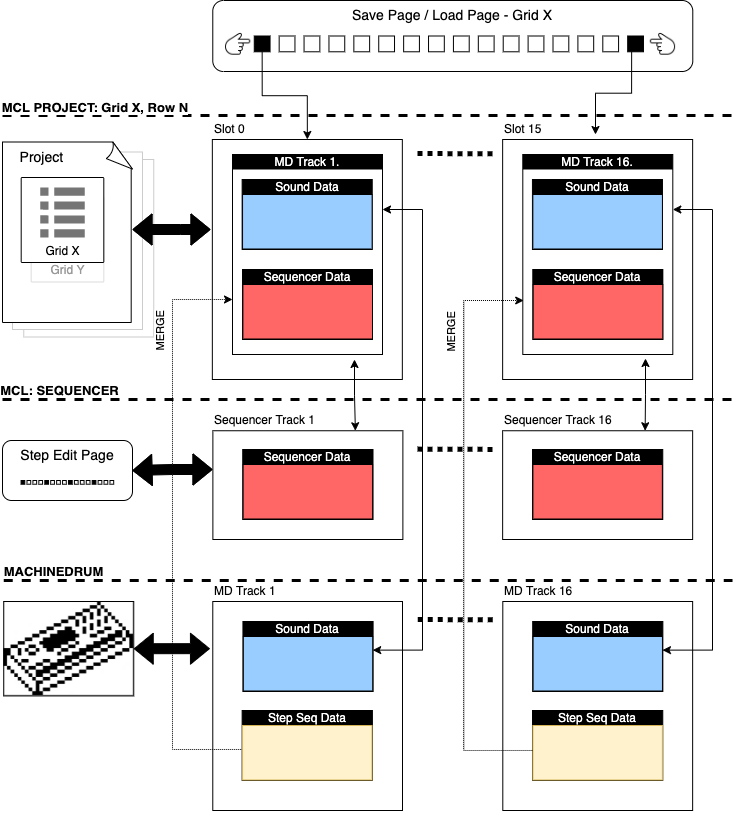
\includegraphics[scale=0.7]{save_or_load_grid_x.png}
    \caption{Save Page / Load Page - Grid X - MD }
    \label{fig:my_label}
\end{figure}
\begin{figure}
    \centering
    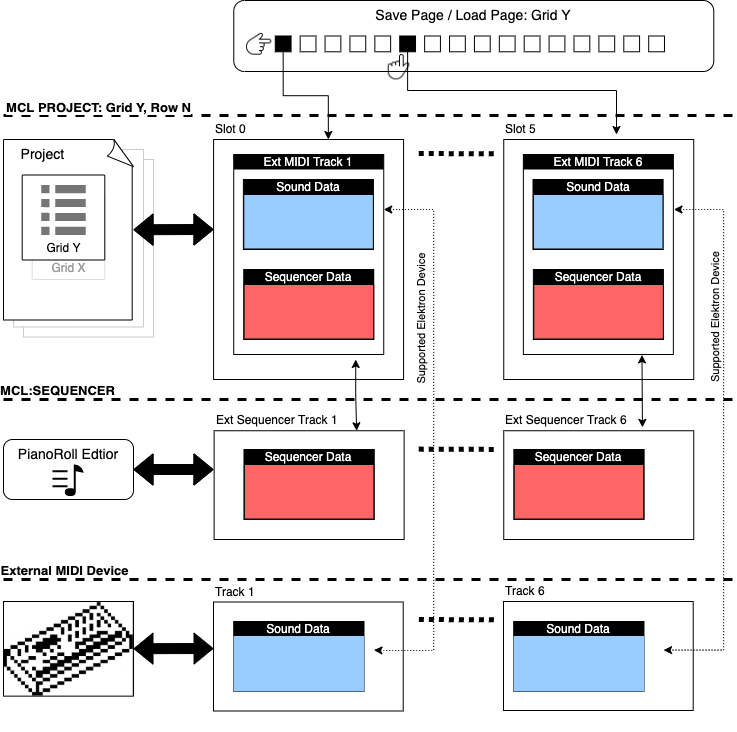
\includegraphics[scale=0.7]{save_or_load_grid_y.png}
    \caption{Save Page / Load Page - Grid Y - External MIDI}
    \label{fig:my_label}
\end{figure}
\begin{figure}
    \centering
    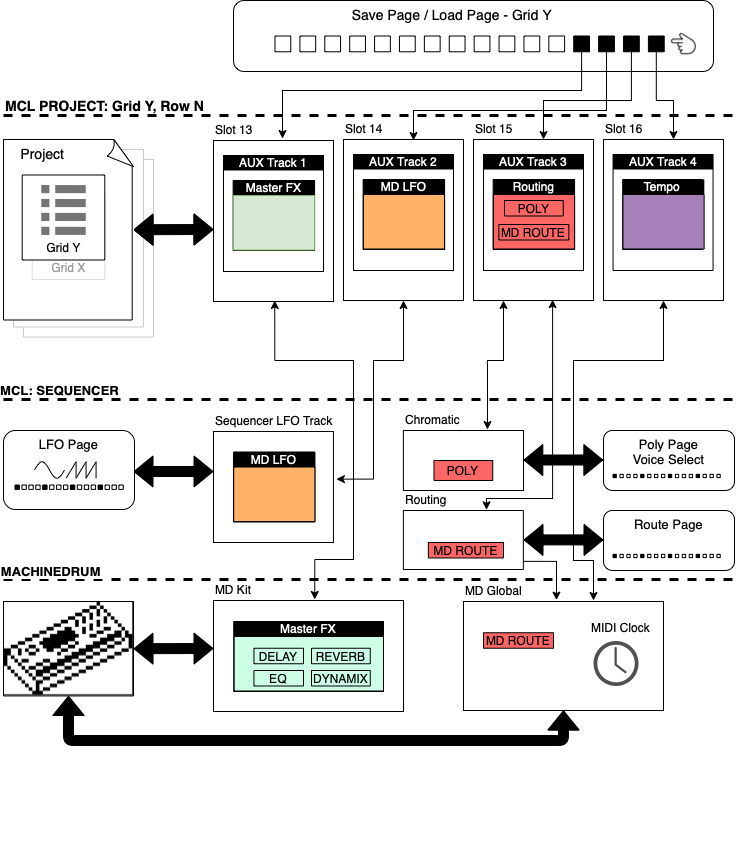
\includegraphics[scale=0.7]{save_or_load_grid_y_md.png}
    \caption{Save Page / Load Page - Grid Y - Auxiliary}
    \label{fig:my_label}
\end{figure}

\chapter{Save Page}

The Save Page is used to save track data to specific slots in the current row of the visible  Grid.\\
\\
Available save modes:
\begin{itemize}
    \item SAVE: Save the MCL's sequencer data and associated device's sound data.
\end{itemize}

\screenshot{save_to_a.png}

\textit{The Save Page is accessible from the GridPage by pressing the \textbf{<Save>} function button. Alternatively, pressing the MD's \textbf{[Function] + [YES]} keys will open the Save Page.}

\encodersbuttons{Mode}{--}{--}{--}{Cancel Save}{Toggle Grid}{--}{Group Select}
\newpage
\section{Saving Individual Tracks}
The Save Page utilises the MD's \textbf{[Trig]} keys to specify which tracks are to be stored. Pressing and releasing multiple \textbf{[Trig]} keys will  save the corresponding sequencer tracks to the matching slots in the current row of the visible Grid.
\section{Grid Toggle}
When in the Save or Load page, the \textbf{<Shift>} button can be used to toggle between Grid X or Grid Y.
\section{Simultaneous Save from Grid X and Grid Y}
It is possible to simultaneously save a collection of tracks from both Grids X and Y. 
\begin{itemize}
\item First select the tracks from Grid X pressing and holding the corresponding \textbf{[Trig]} keys.
\item Tap \textbf{<Shift>} to switch grids
\item Release the \textbf{[Trig]} selection
\item Select tracks from the alternate Grid Y pressing and holding the corresponding \textbf{[Trig]} keys. 
\item Finally release the second grid \textbf{[Trig]} selection to confirm the action. 
\end{itemize}

\section{Save Track Groups:}
When in the Save or Load Page, holding the \textbf{<Shift>} button or MD's \textbf{[YES]} key opens the Group Select menu,
allowing you to load or save all tracks corresponding to a group.\\An entire row/pattern across both Grids X + Y can be loaded or saved this way.\\
\\
There are four groups:
\begin{enumerate}
    \item MIDI Device 1 (MD)
    \item MIDI Device 2 (A4/MNM/Generic MIDI)
    \item FX (MDFX + LFOTrack + RouteTrack)
    \item TEMPO
\end{enumerate}
From the Group Select Menu each group can be enabled/disabled using the MD's \textbf{[Trig]} keys.\\
\\
Releasing \textbf{<Shift> / [YES]} will save tracks corresponding to the active groups.



\chapter{Load Page}
The Load Page is used to load tracks from slots in the current row of the active Grid. When a slot is loaded, Machine/Sound data is sent to the corresponding MIDI device and the sequencer data is loaded into the matching sequencer track.
\screenshot{load_from_a.png}\\
\textit{The Load Page is accessible from the GridPage by pressing the MD's \textbf{[Enter/Yes]} key.}
\encodersbuttons{Load MODE: [ MAN, AUT, QUE ]}{Length Override: [ -, N ]}{--}{ Quantization}{Cancel Load}{--}{--}{Group Select}\\
\textit{The Length and Quantization encoders can be toggled between exponential and incremental value changes by holding down the encoder button when rotating.}
\\\\
The MD's \textbf{[Bank A/B/C]} keys can be used to quickly change the load MODE setting between [ MAN, AUT, QUE ].
\newpage
\section{Loading Individual Tracks}
The Load Page utilises the MD's \textbf{[Trig]} keys to specify which slots are to be loaded. Pressing and then releasing multiple \textbf{[Trig]} keys will load the corresponding slots from the current row of the visible Grid.
\section{Grid Toggle}
The \textbf{[Scale]} button can be used to toggle loading between Grid X, the 16 MD tracks, or Grid Y, the EXT (1-6) and AUX (12-16) tracks.
\textbf{[Trig]} keys.
\section{Simultaneous Load from Grid X and Grid Y}
It is possible to simultaneously load a collection of tracks from both Grids X and Y. 
\begin{itemize}
\item First select the tracks from Grid X pressing and holding the corresponding \textbf{[Trig]} keys.
\item Tap \textbf{[Global]} to switch grids
\item Release the \textbf{[Trig]} selection
\item Select tracks from the alternate Grid Y pressing and holding the corresponding \textbf{[Trig]} keys. 
\item Finally release the second grid \textbf{[Trig]} selection to confirm the action. 
\end{itemize}

\section{Load Track Groups}
When in the Save or Load Page, holding the MD's \textbf{[Enter/Yes]} key opens the Group Select menu, allowing you to load or save all tracks corresponding to a group. An entire row (pattern) including tracks across both Grids X + Y can be loaded or saved this way.\\\\
\screenshot{group_select_page.png}
There are five groups:
\begin{enumerate}
    \item MACHINEDRUM \textit{(Grid X tracks 1-16) + MDFX (\textbf{FX} = Grid Y track 13)}
    \item EXT MIDI DEVICE (A4/MNM/Generic MIDI) \textit{(Grid Y tracks 1-6)}
    \item PERF \textit{(\textbf{PF} = Grid Y track 12) + LFOTrack (\textbf{LF }= Grid Y track 15) }
    \item  RouteTrack \textit{(\textbf{RT} = Grid Y track 14) }
    \item TEMPO \textit{(\textbf{TP} = Grid Y track 16)}
\end{enumerate}
From the Group Select Menu each group can be enabled/disabled using the MD's \textbf{[Trig]} keys 1-5. \\
\\
Releasing \textbf{[Enter/Yes]} will load tracks corresponding to the active groups.

\section{Playback Queue}
Each column of the grid has a dedicated Playback Queue.\\\\Up to 8 slots can be queued in each column.  The slots in the queue form a repeating chain, each slot will be loaded sequentially. When the end of the queue is reached the first slot is loaded again.\\\\Queued slots are drawn with inverse colours on the Grid Page.\\\\The Playback Queue for any column can be activated by setting the load MODE to QUE and then loading a slot in that column.

\section{LOOP \& JUMP}
Each slot contains a LOOP \& JUMP setting which can be adjusted via the Grid page's Slot Menu.\\\\The LOOPS value specifies how many times a track should repeat before it transitions to the slot located at the the bank \& row specified by JUMP.
\\\\The LOOP \& JUMP settings only applies when a slot is loaded with load MODE set to: Auto (AUT). Auto mode is a useful way to create preset arrangement or songs.

\section{Load MODE setting}
Each column of the grid has a dedicated MODE setting. The MODE setting is applied to the corresponding column on load, and can be set to one of the following values:

\begin{itemize}
    \item Manual (MAN):  The selected slots will be loaded at the next transition interval. Existing playback queues in matching columns will be discarded.
    \item Auto (AUT): The selected slots will be loaded at the next transition interval. If the slots LOOP setting is greater than 0, the column will begin loading slots automatically based on their LOOP/JUMP settings. Existing playback queues in matching columns will be discarded.
    \item Queue (QUE): Each slot will be added to the corresponding column's playback queue. The slots in the queue will be loaded sequentially and repeat in a loop. A maximum of 8 slots can be queued per column. 
\end{itemize}

As each column has an independent mode setting, it is possible to have some slots loading automatically (AUT) according to their LOOP \& JUMP setting, other slots can be looping in an improvised queue (QUE) the remaining slots could be left static via manual load (MAN).
\newpage
\section{Slot Length Override}
When load mode is set to QUE, the LEN parameter allows overriding the loaded slot's length. This can be useful if you have a short track, of say 4 steps, and instead want it to play for 16, looping throughout. Alternatively if you are loading a group of slots, each with different length, it is possible to force them to all play to the same length.

\section{Quantization Rules}
The quantization rules specify the transition interval for the selected slots.\\
The minimum quantization value is 2 steps. Quantization values can be changed by adjusting the "Q:" parameter, and increase in powers of 2. Holding down the encoder button will step increment the quantization value.
\begin{itemize}
\item 02: Toggle cue on next possible 2nd step
\item 04: Toggle cue on next possible 4th step
\item 08: Toggle cue on next possible 8th step 
\item 16: Toggle cue on next possible 16th step 
\item 32: Toggle cue on next possible 32th step 
\item 64: Toggle cue on next possible 64th step
\end{itemize}
\section{Load Destination}
\screenshot{load_destination.png}
In Manual mode, pressing the \textbf{[ Function ]} key from the Load Page will allow you to specify a DESTINATION track for the next load. The offset track is chosen by pressing a \textbf{[ Trig ]} key.
\section{Track Levels}
\textit{To provide consistent level mixing across slot loading, the LEV parameter of a loaded track is never transmitted when the sequencer is running.}\\\\This allows the performer to use the LEV parameter to fade the loaded track in and out of the mix. The MD's track's VOL parameter should therefor be used to control the relative track loudness.\\\\
\textit{Please read the manual section describing the \textbf{Config-->Machinedrum-->Normalize} setting which automatically adjusts a saved track's gain staging for this purpose.}

\chapter{Additional Loading Methods}
\section{Loading via [Bank] + [Trig]}
The Machinedrum's pattern changing functionality has been replicated in MCL. Each row of the Grid can be imagined as a pattern, compromising of slots for each of the MD's 16 tracks, plus Auxiliary slots containing the Master FX settings.

\begin{itemize}
   \item A combination of \textbf{[Bank]} + \textbf{[Trig]} will load the corresponding row of the grid.\\\\ \textit{Slots are loaded from the chosen row, according to the Load Page's Group Selection settings. If the MD groups is active, this mimics the behaviour of pattern loading on the MD.}
   \item A combination of \textbf{[Bank]} + multiple \textbf{[Trig]} will chain multiple rows together.\\\\\textit{This is achieved by automatically setting each column's load MODE setting to QUE and then adding slots to each Playback Queue.}
\end{itemize}
\section{Loading via the Grid Slot Menu}
Slots can be loaded directly from the Grid Page's Slot Menu.
\begin{itemize}
\item From the Grid Page, pressing and holding the \textbf{[Exit/No]} button will open the Slot Menu. The MD's \textbf{[Up/Down/Left/Right]} keys can then be used to highlight a selection of slots
\item When the Slot Menu is active, selected slots can be loaded by pressing the MD's \textbf{[Enter/Yes]} key.
\item Slots are loaded according to the current load MODE setting. If more than one row is selected, the load MODE is temporarily set to QUE, and the loaded slots are added to each column's Playback Queue.
\item The MD's \textbf{[Bank A/B/C]} keys can be used to quickly change the load MODE setting between [ MAN, AUT, QUE ].
\end{itemize}

\chapter{MCL Sequencer Pages:}

\textit{The primary Sequencer Pages are accessed using the \textbf{PageSelect} page. These include:
\begin{itemize}
    \item (MD) Step Edit Page
    \item (Ext MIDI) PianoRoll Page
    \item (MD/Ext MIDI) Chromatic Page
\end{itemize}}
\section{Track selection}
For the Step Edit and Parameter Edit pages, the current track selection is synced to the Machinedrum. When you change track on the MD the track will change on the MegaCommand.\\\\
For the PianoRoll page, the current track can be selected from the PianoRoll menu's TRACK SELECT option. Alternatively, if an external MIDI device is connected to port 2, the track will automatically change to the first EXT track that is set to the same MIDI channel as incoming note data.
\\\\
\textit{Automatic track select can be disabled from the MCL system menu option Global -> Machinedrum -> TRACK SELECT}
\section{Live Record:}
Live Record mode can be activated from any Sequencer page by pressing \textbf{[ Save ]}.\\Depending upon the page type, live Record can be used to record:
\begin{itemize}
    \item Trig presses
    \item Parameter changes, CC Automation
    \item Notes played in Chromatic Mode
    \item Notes played on the PianoRoll page.
\end{itemize}
Pressing \textbf{[ Load ]} during a recording will clear the sequence for the current track.

\newpage
\section{Track menu}
\screenshot{track_menu.png}

The track menu will be opened when holding \textbf{[ Shift 2 ]}, and the entry activated on release, similar to the slot menu.
The track menu consists of the following entries that are common to all Sequencer Pages:

\begin{figure}[hb]
    \begin{tabular}{|l|l|}
    \hline
    \rowcolor[HTML]{C0C0C0} 
    Entry            & Function                                                        \\ \hline
    Edit     & change editor mode   \\ \hline
    Track Select     & select active track                  *only visible when TRACK SELECT = MAN                                              \\ \hline
    Copy             & \begin{tabular}[c]{@{}l@{}}TRK: copy track, ALL: copy pattern\end{tabular}                                             \\ \hline
    Clear            & \begin{tabular}[c]{@{}l@{}}TRK: clear track, ALL: clear pattern\end{tabular}                                           \\ \hline
    Paste            & \begin{tabular}[c]{@{}l@{}}TRK: paste track, ALL: paste pattern\end{tabular}                                           \\ \hline
    Speed & \begin{tabular}[c]{@{}l@{}}The current track's playback speed\\ 1x, 2x, 3/2x, 3/4x, 1/2x, 1/4x, 1/8x.\\ Hold [ Load ] and release [ Shift 2 ] to change speed of all tracks. \end{tabular}                          \\ \hline
    Shift            & \begin{tabular}[c]{@{}l@{}}L/R: shifts the track left/right.\\ L ALL/R ALL: shifts the pattern left/right.\end{tabular} \\ \hline
    Reverse          & TRK: reverse the track, ALL: reverse the pattern                                                                          \\ \hline
    \end{tabular}
\end{figure}
\chapter{Step Editor Page:}
The Step Editor (StepEdit) page is used to program MCL's internal sequencer for a selected MD track and is fully integrated with the MD's pattern editing user interface.
\screenshot{step.png}\\
\textit{Press \textbf{<Page>/[Global] + [Trig 5]} key to open the StepEdit page.}\\\\
\textit{Pressing the MD's \textbf{[REC]} button will allow you to toggle in and out of the StepEdit page from anywhere within MCL.}
%\fbox{\includegraphics[scale=.40]{seq_step_page.png}}
\screenshot{step_action.png}

\encodersbuttons{Trig Condition}{Micro-Timing}{Track Length}{Note}{Toggles REC}{}{Rotate Sequencer Page | Apply All}{Track/Trig Menu}
\newpage
\section{GUI:}
\begin{itemize}
\item The StepEdit page leverages the MD's GUI for editing.
\item The editing mode can be toggled between Trig, Lock, Mute and Slide by pressing \textbf{[Func] + [Bank C/D/E]}.
\item The 16 steps of the current page for the current track are displayed on the bottom row.
\item The \textbf{[Trig]} buttons on the MD correspond to the visible steps. Pressing a \textbf{[Trig]} will add the step. A press followed by quick release will remove the step. 
\item Trig Conditions and Micro-Timing settings are per step and are set by holding \textbf{[Trig]} and rotating \textbf{<Encoder1>} or \textbf{<Encoder 2>}. Alternatively the MD's \textbf{[Up/Down]} keys can be used to change Trig Conditions and \textbf{[Left/Right]} for Micro-Timing.
\item Parameter locks can be added to a step by selecting a \textbf{[Trig]} and then rotating the corresponding MD \textbf{[Encoder]}.
\item When a parameter lock is set, the step sequencer LEDs will blink on the MD, and the MCL will display a filled rectangle above step trig on screen.
\item Parameter locks can be removed individually by selecting a \textbf{[Trig]} and tapping the MD's matching \textbf{[Encoder]}. All parameter locks can be removed by holding the \textbf{[Trig]} and pressing \textbf{[Clear]} to clear the step.
\item Parameter lock transmission can be disabled for any step by removing the lock step in LOCK editor mode.
\item Trigs and parameter lock transmission can be temporarily disabled by adding a step in MUTE editor mode.
\item A step can be previewed by holding down the matching \textbf{[Trig]} key and pressing \textbf{[Enter]}.
\item The visible sequencer page can be rotated pressing \textbf{<Load | Yes>} or the MD's \textbf{[Scale]} key.
\item The steps of the sequence can be shifted left or right by holding the MD's \textbf{[Func]} key and pressing \textbf{[Left]} or \textbf{[Right]}
\item The MD's \textbf{[Clear/Copy/Paste]} functions work across Track, Sequencer Page and Step.
\item The Length and Speed of the track can be set via the MD's Scale menu by pressing
\textbf{[Func]} followed by \textbf{[Scale]}.

\end{itemize}
\newpage
\section{Trig Conditions:}
\begin{itemize}
\item L1,L2,L3,L4,L5,L6,L7,L8 (For Ln, step is only triggered after every n iterations of track)
\item P10, P25, P50, P75, P90 (For Pxx, step has a xx percent chance of being triggered)
\item 1S. (One Shot trig, step is only triggered once)
\item Each trig condition above has a twin denoted by the \^{} character e.g L1\^{}, L2\^{}, P1\^{}. When these condition modes are selected, parameter locks and slides must also obey the trig condition.
\end{itemize}
\section{Micro-Timing:}
When editing Micro-timing, the uTIMING window will be visible on both the MC and MD. The number of divisions between notes is dependent on the track's Speed setting.\\\\\textit{The MC's sequencer has a resolution of 1/192th per quarter notes}\\
\screenshot{utiming1.png}
\section{Track Speed \& Length:}
All sequencer tracks can be played at an independent speed and length.\\\\
The chosen speed can be one of either: 1x, 2x, 3/2x, 3/4x, 1/2x, 1/4x, 1/8x.\\Triplets can be achieved using either 3/2x, 3/4x.
\begin{itemize}
\item Track speed can be adjusted from MCL's Track Menu.
\item Track length is controlled by rotating \textbf{<Encoder 3>}.
\item To change the lengths of all tracks of the current track type, simultaneously hold down \textbf{<Load>} whilst rotating \textbf{<Encoder 3>}.
\item The MD's "Scale Setup" Menu accessible via \textbf{[Func] + [Scale]} can be used to quickly change the track speed \& length. If the "Scale Setup" menu is opened outside of Step Edit mode, the speed \& length changes will apply to all 16 tracks.
\end{itemize}
\newpage
\section{Change Edit Mode:}
By default, the Step Edit page opens in Trig Edit mode. It is possible to change this edit mode to program the track's sequencer data for either Trigs, Locks, Slides or Mutes.
\begin{itemize}
\item To change the Edit mode, press and hold the \textbf{<Shift>} to open the track menu, rotate \textbf{<Encoder 2>} to the entry \textbf{Edit}, then rotate \textbf{<Encoder 1>} to select one of either Trig, Lock, Slide or Mute.
\item Alternatively, the Edit mode can be rotated between Lock, Mute and Slide by pressing the MD's \textbf{[Func] + [Bank C/D/E]} keys.
\end{itemize}
\section{Clearing a Sequence:}
\begin{itemize}
\item To clear the current track, press and hold the\textbf{<Shift>} to open the track menu, rotate \textbf{<Encoder 2>} to the entry \textbf{CLEAR}, then rotate \textbf{<Encoder 1>} to select \textbf{TRK}.
\item To clear all MD tracks, select \textbf{ALL}
\item The MD's \textbf{[Clear]} function can be used to clear a track, or all track.
\end{itemize}
\section{Rotate Track Page:}
Each track consists of 4 pages of 16 steps, for a total of 64 steps per track.
\begin{itemize}
\item Rotate the visible track page by pressing the \textbf{<Load>} button.
\item The MD's \textbf{[Scale]} button can also be used to rotate the visible track page.
\end{itemize}
\section{Chromatic Step Edit:}
The Step Edit allows you to adjust a step's pitch by setting a note value. 
\begin{itemize}
\item Press and hold trigger button(s) on the MD. Adjusting \textbf{<Encoder 4 >} will allow you change the note value of the selected steps.
\item An external MIDI keyboard connected on Port 2, can be used to select the note.
\item A keyboard will be drawn on the display, showing the current note.
\end{itemize}
\screenshot{step_keyboard.png}
\section{Slides:}
Each parameter lock can be made to slide up or down to the nearest step containing a parameter lock of the same type.
\\\\
To add slides to your sequence change the Edit Mode to "SLIDE" (see above).
\section{Mutes:}
Individual steps of your sequence can be muted, by placing a mute trig at the corresponding position. Mutes are reset on sequencer restart.\\\\ 
To add mutes to your sequence change the Edit Mode to "MUTE" (see above).
\section{Shift Sequence:}
The sequence of an individual track can be shifted left of right. Press \textbf{[Function]} + \textbf{[Left/Right]} on the MD. The sequencer menu can also be used to shift the entire pattern via the SHIFT option.
Similarly you can reverse a track's sequence from the sequencer menu option REVERSE.
\section{Live Record:}
Live Record mode can be activated either by pressing  \textbf{<Save>} or using the MD's \textbf{[Rec]} function. Both trig and parameter locks can be recorded simultaneously.
\section{Step Menu:}

\screenshot{step_menu.png}
The step menu will be opened by selecting one or more step/trig from the TI and when holding \textbf{<Shift>}. The entry activated on release, similar to the slot menu.
The step menu consists of the following entries:

\begin{figure}[hb]
    \begin{tabular}{|l|l|}
    \hline
    \rowcolor[HTML]{C0C0C0} 
    Entry            & Function \\ \hline
    Clear            & Locks: Clear step's parameter locks \\ \hline
    Copy         & Copy step\\ \hline
    Paste        & Paste step\\ \hline
    Mute         & Mute or Unmute step\\ \hline
    \end{tabular}
\end{figure}
\chapter{PianoRoll Editor Page}
The PianoRoll page is used to edit External MIDI sequencer tracks 1-6.\\
The editor features two modes: Note editing and Automation editing.
\screenshot{proll.png}
\\
\textit{Press \textbf{[Bank Group] + [Trig 7]} to open the Pianoroll Editor page}
\encodersbuttons{Cursor X}{Cursor Y / Note Value}{Cursor Width / Note Width }{Zoom}{Record}{PageSelect}{Add or Remove Note}{Pianoroll Menu}
\section{GUI}
\screenshot{proll_edit.png}
The PianoRoll editor operates in continuous time, with the finest resolution being 1/192nd of a quarter note. Dots are drawn to illustrate each quarter note. Vertical lines denote the commencement of a new beat.
\newpage
\begin{itemize}
\item The cursor can be moved to a specific time offset by rotating \textbf{<Encoder 1>}. 
\item \textbf{<Encoder 4>} adjusts the zoom along time the time axis.
\item  The note value is chosen using \textbf{<Encoder 2>}
\item The note width controlled using \textbf{<Encoder 3>}. 
\item Notes can be both entered and deleted by pressing the \textbf{<Load>} button.
\end{itemize}
Alternatively, the MD's GUI can be used to navigate the piano roll, and edit the sequence.
\begin{itemize}
     \item \textbf{[Enter/Yes]} add or remove notes.
     \item \textbf{[Left/Right]} move cursor along time axis.
     \item \textbf{[Enter/Yes] + [Left/Right]} nudge cursor along time axis (fine control).
     \item \textbf{[Exit/No] + [Left/Right]} adjust cursor width.
     \item \textbf{[Enter/Yes] + [Exit/No] + [Left/Right]} nudge cursor width (fine control).
     \item \textbf{[Up/Down]} move cursor along note axis.
     \item \textbf{[Function] + [Up/Down/Left/Right]} cursor fast travel.
     \item \textbf{[Exit/No] + [Up/Down]} zoom in and out.
     \item \textbf{[Clear/Copy/Paste]} clear/copy/paste for track.
      \item \textbf{[Scale]} Toggle sequencer page.
     \item \textbf{[Function] + [Scale]} The MD's scale menu can be used to configure the length and speed of the current track.
     \item The MD's \textbf{[Trig]} keys can be used to position the cursor at step intervals relative to the current page.
\end{itemize}
\section{External MIDI Control}
An external MIDI device connected on Port 2 or USB MIDI can be used to position the cursor's vertical position.
\begin{itemize}
    \item Ensure that the \textbf{Config-->MIDI-->CTRL PORT} is set to the MIDI port your external keyboard/sequencer is connected.
\end{itemize}
\textit{When using an external MIDI keyboard, the octave, and scale mapping can be changed from the Chromatic Page as discussed in the next chapter.}
Holding a note on an external MIDI keyboard, and then pressing the MD's \textbf{[Enter/Yes]} or a \textbf{[Trig]} key, allows individual notes to  be added at the cursor position.
\\\\
Similarly, using a simultaneous combination of the MD's \textbf{[Trig]} keys and an external MIDI Keyboard, chords can be entered into the Note Editor. First play a chord on the Keyboard, then press \textbf{[Enter/Yes]} or a \textbf{[Trig]} key to store the chord at the cursor location.
\section{Live Record}
Live Record mode can be activated using the MD's \textbf{[Rec]} function. Both note and automation data can be recorded simultaneously. Automation data includes all ControlChannel, Pitchbend and channel pressure messages received on MIDI port 2.\\\\All 6 tracks can be recorded to simultaneously.\\
\\Tracks will only record incoming data that is on the same MIDI Channel. \textit{(see section MIDI Channel Selection)}\\\\
To disable Automation Recording use the CC Rec option in the Track Menu.
\section{PianoRoll Editor Track Menu}
\screenshot{proll_menu.png}
Holding \textbf{[Global]} opens the Track menu. For each track you can adjust the MIDI Channel, track length and playback speed. Cursor editing options are also included here including note velocity and note conditional settings.

\begin{figure}[hb]
    \begin{tabular}{|l|l|}
    \hline
    \rowcolor[HTML]{C0C0C0} 
    Entry        & Function \\ \hline
    Track Select & Change Track \\ \hline
    Edit         & Note or Automation editing modes\\ \hline
    VEL         & Note Velocity\\ \hline
    Cond        & Trig Condition\\ \hline
    Channel     & MIDI Channel\\ \hline
    Key         & MIDI Channel\\ \hline
    CC Rec      & Enable/Disable Automation recording.\\ \hline
    \end{tabular}
\end{figure}
\section{Ext MIDI Track Selection \& Mutes}
When opening the Track Menu \textbf{[Global]} from within in either the PianoRoll Editor or Chromatic Page, the MD's \textbf{[Trig]} keys can be used to switch between Ext MIDI Tracks and/or mute/unmute them. 
\begin{itemize}
    \item MD \textbf{[Trig]} keys 1-6 correspond to Ext MIDI Track selection 1-6.
    \item MD \textbf{[Trig]} keys 9-14 correspond to Ext MIDI Track mutes 1-6.
\end{itemize}

\section{MIDI Channel Selection}
Each Ext MIDI track listens and transmits on a set MIDI Channel. The channel defaults to the track number. This can be easily changed by modifying the Track menu CHAN option.\\
\section{Change Edit Mode}
From the PianoRoll menu, the "Edit" parameter changes the editing mode. Switch between either Note editing, or editing automation parameters 1-8.
\newpage

\section{Automation Editing}
\screenshot{proll_aut.png}
\textit{The PianoRoll Editor page allows for automation editing. From the Track menu, use the "Edit" menu option to select one of eight Automation Parameters.}
\\\\
Each External MIDI track features 8 automation parameters.\\
\section{Automation Editor Track Menu}
Hold \textbf{[Global]} to open the Track menu.
\begin{figure}[hb]
    \begin{tabular}{|l|l|}
    \hline
    \rowcolor[HTML]{C0C0C0}
    Entry        & Function \\ \hline
    Edit         & Note or Automation editing modes\\ \hline
    Slide      & Linear slide between automation values \\ \hline
    CC         & CC destination, Program Change, Pitch Bend, Channel Pressure,  MIDI learn \\ \hline
    CC Rec      & Enable/Disable Automation recording.\\ \hline
    \end{tabular}
\end{figure}
\\
Slide: enables/disable interpolation between automation events.\\\\
CC: Allows a specific MIDI Control Channel number to be a chosen parameter.
\begin{itemize}
    \item When set to LEARN, to Automatically learn the next received CC on the same MIDI channel.
    \item When set to PRG, the track will send Program Change messages.
    \item When set to PB, the track will send pitch bend messages.
    \item When set to CHP, the track will send channel pressure messages.
\end{itemize}

\section{Automation Step Locks}
It's possible to enter CC automation data at specific steps, by holding down the corresponding \textbf{[Trig]} and rotating the external MIDI CC control knob. This feature is available from both the Piano Roll and Automation Editor.



\chapter{Chromatic Page:}
The Chromatic Page, enables the user to play tracks of the Machinedrum or an External MIDI device chromatically. Each MD track can be used as a voice of a monophonic/polyphonic synthesizer. Melodic compositions can be recorded in real-time.
\screenshot{chroma.png}\\
\textit{The Chromatic page can be accessed by pressing \textbf{<Page>/[Global]} and \textbf{[Trig 8]}.}
\\
\section{Using the Chromatic Page:}
\screenshot{chromat_action.png}
\encodersbuttons{Octave (OC)}{Fine Tune (F)}{Track Length}{Scale Type (S)}{Record}{PageSelect}{Apply All}{Track/Trig Menu}
The top left of the screen shows the active device tab and indicates whether the Chromatic Page is targeting the MD or an Ext MIDI device.
The Octave (OCT) parameter allows for adjusting the relative octave of the track's tuning. The Detune (DET) parameter can be used for offsetting the absolute pitch by small increments (MD only). Length (LEN) controls the length of the associated sequencer track. Scale (SCA) maps MIDI notes to a musical scale type.
A keyboard at the bottom of the screen is displayed showing notes as they are played.
\newpage
\section{Setup for Chromatic mode:}
There are two important configurations options that must be understood in order to use the Chromatic Page correctly:
\begin{itemize}
    \item The \textbf{Config-->Machinedrum-->CTRL CHAN} parameter determines whether the MD should receive note input from the MD's \textbf{[Trig]} keys, or from a MIDI channel on an External MIDI Device. \textit{See Chapter: Global Settings}
    \item The PolyPage is used to allocate one or more MD tracks as dedicated synth voices. \textit{See Chapter: Polyphonic Mode} 
\end{itemize}

\section{Tuning:}
For MD tracks hosting a supported machine, the machines’s pitch is tuned to notes of a selected scale. The track can then be played using the MD's \textbf{[Trig]} keys or an attached MIDI keyboard.\\\\
The Machinedrum X.05 OS allows for more precise tuning of machines. If the machine's tuning setting is TONAL then the new quarter tone, equal temperament tuning table will be used. If the machine's tuning setting is DEFAULT the legacy microtonal tuning table is used.
\\
\section{Chromatic Page Track Menu:}
\screenshot{chromatic_menu.png}
Holding \textbf{[ Shift 2 ]} opens the Track menu.
\begin{figure}[hb]
    \begin{tabular}{|l|l|}
    \hline
    \rowcolor[HTML]{C0C0C0} 
    Entry            & Function \\ \hline
    Arpeggiator      & Opens the Arpeggiator Page \\ \hline
    Transpose        & Transpose scale by semi-tone\\ \hline
    Polyphony        & Opens the PolyPage, for voice selection\\ \hline
    \end{tabular}
\end{figure}
\newpage
\section{Ext MIDI Tracks:}
The Chromatic Page is also used to record/play the External MIDI tracks.
Octave and Scale settings from the Chromatic Page are also applied to incoming note data when using the PianoRoll editor.
\section{Ext MIDI Track Selection \& Mutes:}
When opening the Track Menu \textbf{<Shift>} from within in either the PianoRoll Editor or Chromatic Page, the MD's \textbf{[Trig]} keys can be used to switch between Ext MIDI Tracks and or  mute/unmute them.
\begin{itemize}
    \item MD \textbf{[Trig]} keys 1-6 correspond to Ext MIDI Track selection 1-6.
    \item MD \textbf{[Trig]} keys 8-12 correspond to Ext MIDI Track mutes 1-6.
\end{itemize}
\section{Recording a Sequence:}
\textit{Press the \textbf{<Save>} button ot use the MD's \textbf{[Rec]} function to enable live record mode.\\}

Play notes on either the MD or External Midi to record a melody.

\section{Clearing Recorded Sequence:}
\begin{itemize}
\item To clear the current track, press and hold the\textbf{<Shift>} to open the track menu, rotate \textbf{<Encoder2>} to the entry \textbf{CLEAR}, then rotate \textbf{<Encoder1>} to select \textbf{TRK}.
\item To clear all tracks of the current track type, select \textbf{ALL}.
\item A recorded track can be quickly cleared using the MD's \textbf{[Clear]} function.
\end{itemize}

\section{Track Speed and Length:}
\begin{itemize}
\item Track length is controlled by rotating \textbf{<Encoder 3>}.
\item To change the lengths of all tracks of the current track type, simultaneously hold down \textbf{<Load>} whilst rotating \textbf{<Encoder 3>}.
\item Speed and length can be set via the Track menu, by holding \textbf{<Shift>}.
\item For the Machinedrum, track speed and length can also be set using the MD's Scale menu by pressing \textbf{[Func] + [Scale]}.
\end{itemize}
\newpage
\section{External MIDI Device:}
Melodies and chords can be played and recorded from an External MIDI device on port 2.
\\

When MIDI note data is received, MCL will switch to the first Exteral MIDI sequencer track that has the same MIDI channel.
\\

\textit{The active device illustrated in the top left corner of the display, will switch over from MD to MI, when MIDI notes are received.}
\\
\chapter{Polyphonic Mode}

\section{Voice Select Page}
The voice select page is used to allocate MD tracks as polyphonic voices.\\
\fbox{\includegraphics[scale=.40]{voice_select_page.png}}\\\\
\textit{To open the voice select page: Enter \textbf{Config-->Machinedrum-->Poly Config}.\\Alternatively press \textbf{<Save>} + \textbf{<Load>} from  Chromatic Page, or access via the Chromatic Page's Track Menu item \textbf{"POLYPHONY".}}
\section{Voice Assignment:}
MD track's 1-16 can be assigned as polyphonic voices by pressing the matching \textbf{[Trig]} keys.
\section{Saving/Loading:}
The polyphonic voice selection can be saved and loaded from Grid Y in Auxiliary slot 14 (Route) along with audio Routing configuration. In addition, polyphonic voice selection is automatically retained across power on/off.
\\\\
\textit{For more information on slot positions and their corresponding tracks see  "Sequencer: Saving and Loading".}
\section{Voice Modes:}
When in the Chromatic Page, the Machinedrum's current active track will be used as a monophonic voice.\\
\\
If the current active track is part of the Polyphonic track selection POLY mode will be activated. In this mode the MD will be played polyphonically using voices selected from the POLY Page.\\
\\
When POLY mode is active, tracks become 'linked'. Track length and parameter changes will be synchronised across the voices. Clearing a polyphonic track via the MD's \textbf{[Clear]} function will clear all polyphonic tracks.
\newpage
\section{Getting started with Poly Mode}
For best results, make sure that the tracks allocated as a poly voice are all set to the same machine type on the MD. You can quickly copy one track to another using the MD's \textbf{[Copy ] / [Paste]} functions.\\\\
Use the MD's \textbf{[Encoder]} wheel to focus on on the allocated poly voices.\\
Enter the Chromatic page, press the \textbf{[Trig]} buttons to be begin playing the MD polyphonically.
\section{Machinedrum External MIDI}
The MD can be played chromatically using an attached MIDI keyboard/sequencer connected to MIDI input port 2.\\\\
To enable/disable control from an external device you must change the MCL's \textbf{Config-->Machinedrum-->CTRL CHAN} setting from INT (internal) to a desired MIDI channel or OMNI (all channels).\\
\\
When external control mode is enabled, the MD's \textbf{[Trig]} keys will be disabled.\\\\
\subsection{MIDI CC:}
You can control the voice parameters by sending MIDI CC messages via an External MIDI controller to port 2.\\\\CC 16 to 39 control MD parameters 1 to 24 on the active track, or across all polyphonic tracks.


\chapter{Arpeggiator Page:}
The Arpeggiator Page allows control of each track's dedicated Arpeggiator. Arpeggiator settings are not retained when saving or loading tracks, the generated sequence can however be recorded to the track in realtime.
\screenshot{chro_menu.png}
\\
\textit{To enter the Arpeggiator Page: From the Chromatic Page, enter the Track Menu by holding \textbf{<Shift>} or \textbf{[Global]} then select Arpeggiator. }

\screenshot{arp_page.png}
The Arpeggiator has 3 states of operation:
\begin{enumerate}
    \item -- (Off)
    \item ON
    \item LATCH (Notes are held down)
\end{enumerate}

When enabled, the arpeggiator will  play when the sequencer is running. 
\encodersbuttons{ARP State (ARP))}{Mode}{Rate (speed)}{Range (octave)}{}{}{}{}

\section{Arpeggiator Modes:}
\begin{tabular}{|l|l|}
\hline
\rowcolor[HTML]{C0C0C0} 
MODE                                  & Notes played in order:                                                                                                                                                                        \\ \hline
UP                                    & Ascending                                                                                                                                                    \\ \hline
DOWN (DWN)                           &  Descending                                                                            \\ \hline

UP DOWN (UD)                 &  Ascending Descending                                                                                                                                                                   \\ \hline
DOWN UP (DU)                   & Descending Ascending                                                                                                                                                                  \\ \hline
UP AND DOWN (UND)                 & Ascending and then Descending                                                                                                                                                                 \\ \hline
DOWN AND UP (DNU)                & Descending and then Ascending                                                                                                                                                                   \\ \hline
CONVERGE (CNV)                & Converging                                                                                                                                                                      \\ \hline
DIVERGE (DIV)                & Diverging                                                                                                                                                                 \\ \hline
CONVERGE AND DIVERGE (CND)     & Converging Diverging                                                                                                                                                           \\ \hline
PINKY UP (PU)                & Ascending with first note played before every other note                                                                                                                             \\ \hline
PINKY DOWN (PD)                & Descending with first note played before every other note                                                                                                                                                                   \\ \hline
THUMB UP (TU)                & Ascending with last note played before every other note                                                                                                                                     \\ \hline
THUMB DOWN (TD)                & Descending with last note played before every other note                                                                                                                         \\ \hline
UP PINKY  (UPP)                & Ascending with only first note increased in octave                                                                                                                                                                 \\ \hline
DOWN PINKY (DP)                & Descending with only first note increased in octave                                                                                           
                                       \\ \hline
UP 2ND (U2)                & Ascending with every second note increased in octave.                                                                                             
                                       \\ \hline
DOWN 2ND (D2)                & Descending with every second note increased in octave. 
                                       \\ \hline
RANDOM (RND)                & Random                                                                                                                   
                                       \\ \hline
\end{tabular}

\chapter{Mixer Page:}
The mixer page displays the audio levels, or parameter values of the sixteen MD tracks of the current Kit.
\screenshot{mixer_page_init.png}

\textit{The Mixer Page is accessible by pressing \textbf{<Page> + [Trig 2]}}

\encodersbuttons{Level}{FLTF (Filter Frequency)}{FLTW (Filter width)}{FLTQ (Filter resonance)}{Solo}{PageSelect}{Mute}{Recall}

The MD's \textbf{[Trig]} keys are is used in conjunction with \textbf{<Encoder 1>} to raise or lower the volume of multiple tracks simultaneously. The remaining encoders can be used to adjust the filter parameters of the selected tracks.\\\\
\textit{The Machinedrum \textbf{[Encoder]}s can be used to manipulate any specific parameter across selected tracks, similar to the MD's built in CTRL-ALL functionality.}
\section{Recall Tracks}
\textit{Selecting a MD \textbf{[Trig]} and pressing either \textbf{<Shift>} or \textbf{[No]} will reset the parameters of each track to the value set during their last load.}
\section{Audio Mutes}
The top row of mixer page shows the Audio Mute state of each Track. The audio mute state changes the audio routing of muted tracks. When a track is muted from the Mixer Page, audio is routed to the Audio Output specified on the Route Page.\\
\\
\textit{Audio mutes are independent from the MD's sequencer mute page.}
\\\\
\section{Mute Tracks}
Holding down \textbf{<Load>} and pressing a trigger buttons on the MD allows you to quickly toggle the mute state of a track.
\section{Solo Tracks}
Holding down \textbf{<Save>} and pressing the trigger buttons on the MD allows you to quickly solo selected tracks.\\\\


 \chapter{Route Page:}
 The Route Page is used to direct the audio of a specific MD track to a selected output.\\\\\textit{Routing configuration can be either stored or recalled by saving or loading to the corresponding Auxiliary track Route slot.} \\
 
\screenshot{route.png}
\textit{The Route page can be accessed by pressing \textbf{[Bank Group]} and \textbf{[Trig 4]}.}
%\fbox{\includegraphics[scale=.40]{route_page.png}}

\encodersbuttons{Output Selection}{--}{Quantization}{--}{--}{PageSelect}{--}{--}

\textbf{<Encoder 1>} can be used to select the audio output destination. The destination can be one of MD's external outputs C, D, E, F.

The MD's \textbf{[Trig]} keys are used to toggle the output of selected tracks, between Main Outputs and the chosen external output.

\screenshot{route_action.png}
\newpage
\section{Quantization Rules:}
The quantization rules specify the timing of the routing changes so that they are in sync with the sequencers.\\
The minimum quantization value is 2 steps. Quantization values can be changed by adjusting
the ”Q:” parameter, and increase in powers of 2. Holding down the encoder button will step
increment the quantization value.
 \begin{itemize}
\item --: No quantization.
\item 02: Toggle cue on next possible 2nd step
\item 04: Toggle cue on next possible 4th step
\item 08: Toggle cue on next possible 8th step 
\item 16: Toggle cue on next possible 16th step 
\item 32: Toggle cue on next possible 32th step 
\item 64: Toggle cue on next possible 64th step
 \end{itemize}
 
 \section{Saving/Loading:}
The routing configuration can be saved and loaded from Grid Y in Auxiliary slot 14 (Route) along with Polyphonic configuration. In addition, routing is automatically retained across power on/off.\\\\
\textit{For more information on slot positions and their corresponding tracks see  "Sequencer: Saving and Loading".}

 
 
\chapter{LFO Page:}
The MCL firmware is equipped with its own LFO modulation source, and controls both track parameters and master FX parameters.\\\\\textit{LFO settings can be either stored or recalled by saving or loading to the corresponding Auxiliary track LFO slot.}

\screenshot{lfo.png}
\textit{To enter the LFO Page: press and hold \textbf{<Page>/[Global]}, then press \textbf{[Trig 4]}.}
\buttons{Toggle LFO ON/OFF}{PageSelect}{Toggle MOD/DST}{LFO Mode}\\
By default the LFO engine is deactivated. To toggle it ON, press \textbf{< Save>}.
\section{Modulation Source}

The modulation source shape, speed and depth can be controlled. The subpage index will show as ``LFO>MOD'' on the left information panel.

\screenshot{lfo_action.png}

\newpage

\encoders{Waveform}{LFO Speed}{Target 1 Depth}{Target 2 Depth}

\section{Modulation Target}
To switch to the Modulation Target subpage, press \textbf{<Load>}. The subpage index will show as ``LFO>DST'' on the left information panel.

\screenshot{lfo_dest.png}

Only valid parameter types for the current target track will be shown for Encoder2/Encoder4. Master FX machines are regarded as individual tracks, each with its own modulation target parameter types. This extends the mastering capabilities of MD, for that one can use the LFOs to create sidechain-like effects etc.

\encoders{Target Machine 1}{Param Type 1}{Target Machine 2}{Param Type 2}

\section{LFO Operation Modes}

The LFO engine operates in different modes, namely \textbf{FREE}, \textbf{TRIG}, \textbf{ONESHOT}.\\Use \textbf{<Shift>} to switch between them.
\begin{itemize}
    \item FREE: Free-running LFO.
    \item TRIG: The LFO is reset on each trig.
    \item ONESHOT: The LFO is reset each trig but only plays through one cycle
\end{itemize}
\section{Parameter Offset}
The LFO modulation is relative to the destination parameter's original value (the lfo offset). The LFO offset will automatically be updated by adjusting the corresponding parameter on the MD's parameter page. For FX parameters it is best to adjust the offset from the FX Pages as changes in the MD FX page will not be immediately received by the MC.
\chapter{Sound Manager Page:}
The Sound Manager page is used to manage the following types of sounds: 
\begin{enumerate}
    \item \textbf{SOUND} -- a sound preset, including the machine assignments, and its associated parameters. It can consist of machine settings from a single track, or two tracks linked by TrigGroup.
    \item \textbf{WAV} -- (UW models only) $.wav$ PCM samples.
    \item \textbf{SYSEX} -- (UW models only) $.syx$ Midi SDS samples, like the ones in the official Machinedrum sound packs.
\end{enumerate}
You can load and save these sounds between the Machinedrum and the Megacommand's micro SD card.

\screenshot{sound_manager.png}
\textit{To enter the Sound Manager Page: press and hold \textbf{<Page>/[Global]}, then press \textbf{[Trig 9]}.}

\section{Navigating the Sound Browser Page.}

The user interface consists of two panels. The currently active sound type is displayed on the left, and a file browser on the right. When the save action is supported by a sound type (currently \textbf{SOUND} and \textbf{WAV} are supported), the [SAVE] entry will also be shown in the file browser panel.

%\fbox{
\includegraphics[scale=.40]{sound_page.png}}
\screenshot{sound_page.png}

Rotate \textbf{<Encoder 1>} to switch between different sound types.\\
Rotate \textbf{<Encoder 2>} to iterate through the files.\\
Press \textbf{<Load>} to enter a directory, or make your selection.\\
Press \textbf{<Save>} to exit/cancel.\\
\\
Note that the file browser will filter the directory content based on the active sound type. For example, if you select \textbf{WAV}, only $.wav$ files will be shown.
 
\section{Saving Sounds}
Save means from MD to MC.\\
To save a \textbf{SOUND}:
\begin{enumerate}
 \item Select the desired track on the MD.
 \item From the Sound Manager, select \textbf{SOUND} in the left panel.
 \item Select [SAVE] in the right panel.
 \item From within the MD, two tracks can be linked by configuring the TrigGroup settings on one, to trigger the other. When two tracks are linked, both the source and destination track machine settings will be stored together to form a single sound.
\end{enumerate}
To save a \textbf{WAV}:
\begin{enumerate}
    \item From the Sound Manager, select \textbf{WAV} in the left panel.
    \item Select [SAVE] in the right panel.
    \item The file browser panel will now display the sample slots in the MD, with ROM slots first, and RAM slots (shown as R1-R4) in the end.
    \item Select the slot to receive sample from.
    \item The SDS dump will be converted to a PCM wave file on the fly, and saved to the micro SD card.
\end{enumerate}

\section{Loading Sounds}
Load means MC to MD.\\
To load a sound, select the sound file the from the file browser panel.\\
For \textbf{WAV} and \textbf{SYSEX}, the file browser panel will now display the ROM slots in the MD, and you can select one slot to send the sample to.

\section{Delete or Rename Sounds:}
\screenshot{file_menu.png}
\textit{From within the Sound Browser, press and hold \textbf{<Shift>} to access the file options menu.}\\\\
From the file options menu, you may delete or rename sound files or create new directories.\\
Use the encoder to make your selection, release \textbf{<Shift>} to activate your choice.

\chapter{FX Delay Page}
Controls the master FX Delay settings.\\
\vspace{-16pt}
\screenshot{delay.png}
\vspace{-32pt}
\paragraph{}\textit{To enter the FX Delay Page: hold \textbf{<Page>/[Bank Group]}, then press \textbf{[Trig 13]}.}
\vspace{-16pt}
\paragraph{}
All the parameters of the delay effect can be controlled. Four of them are displayed at once on screen. Press the \textbf{<Save>} button to toggle between the two groups.

\vspace{-4pt}
\section{FX A}
\vspace{-16pt}
\encoders{Modulation(MOD)}{Modulation Frequency(MFQ)}{Mono(MON)}{Level(LEV)}
\vspace{-25pt}
\screenshot{delay_action_2.png}
\vspace{-10pt}
\section{FX B}
\vspace{-16pt}
\encoders{Delay Time(TIM)}{Delay Feedback(FB)}{Filter Frequency(FLF)}{Filter Width(FLW)}
\vspace{-25pt}
\begin{figure}[h!]
    \fbox{\includegraphics[scale=.40]{delay_action.png}}
\end{figure}

\chapter{FX Reverb Page}
Controls the master FX Reverb settings.\\
\vspace{-16pt}
\screenshot{reverb.png}
\vspace{-32pt}
\paragraph{}\textit{To enter the FX Reverb Page: hold \textbf{<Page>/[Bank Group]}, then press \textbf{[Trig 14]}.}
\vspace{-16pt}
\paragraph{}
All the parameters of the reverb effect can be controlled. Four of them are displayed at once on screen. Press the \textbf{<Save>} button to toggle between the two groups.

\vspace{-4pt}
\section{FX A}
\vspace{-16pt}
\encoders{Damping(DMP)}{Gating(GAT)}{Pre-delay(PRE)}{Level(LEV)}
\vspace{-25pt}
\screenshot{reverb_action_2.png}
\vspace{-10pt}
\section{FX B}
\vspace{-16pt}
\encoders{Decay Level(DVL)}{Decay(DEC)}{Low Pass Filter(HP)}{High Pass Filter(LP)}
\vspace{-25pt}
\begin{figure}[h!]
    \fbox{\includegraphics[scale=.40]{reverb_action.png}}
\end{figure}

\chapter{RAM Page:}
A RAM page is used to automate the recording and playback of the MD's RAM machines. The MCL firmware is equipped with two RAM Pages.
\\\\
A RAM page can be used to sample the MD main outputs or the External Inputs in either Mono or Stereo. The recorded loop can then be played.
Slicing with the various 'slice modes' allows for interesting musical and performance effects.
\\\\
RAM Page 1 will record and playback on MD track 15\\
RAM Page 2 will record and playback on MD track 16\\
\\
\textit{When stereo mode is enabled from \textbf{Configuration-->Aux Pages-->RAMPage}, the recording and playback of RAM machines on track 15 + 16 are linked.}
\screenshot{ram1.png}
\\
\textit{To enter RAM Page one or two: \\Press and hold
\textbf{<Page>}, then press \textbf{[Trig 15]} or \textbf{[Trig 16]}.}
\screenshot{ram1_action.png}

\encoders{Record Source}{Slice Modulation}{Number of Slices}{Record/Playback Length}
\buttons{Record}{PageSelect}{Play}{Slice Mode Toggle}
\newpage
\section{Recording:}
\begin{itemize}
    \item{To use the RAM Machines, first start playing a pattern on the MD.}
    \item{Leave tracks 15 + 16 available as these will be overwritten for RAM machine sampling and playback.}
    \item{From the RAM Page, choose the recording source. INT for sampling the MD internal sound engine. Select the recording length and press \textbf{<Save>} to initiate recording. Recording is quantized with respect to the chosen length.}
    \item The status text "Queue" will be displayed indicating that record event is about to occur. The status text "Recording" will be displayed indicating that the RAM machines are recording. Recording is continuous and can only be stopped by initiating playback.
\end{itemize}

\section{Playback:}
\begin{itemize}
\item Press \textbf{<Load>} to initiate playback. The status text "Queue" will be displayed indicating that play event is about to occur. 
\item The status text "Playback" will be displayed indicating that the RAM machine(s) are playing. Playback is continuous until recording is re-initiated. 
\end{itemize}


\section{Mono:}
When in Mono mode RAM machines can either sample a mono MIX of the MD output, or external inputs A or B
\section{Stereo:}
When in Stereo mode RAM machine one will record MD output A and RAM machine 2 will record MD output B. Similarly if the recording source is set to EXT RAM machine one will record EXT input A and RAM machine 2 will record EXT input B

On playback stereo tracks are panned and linked. Parameter changes across tracks 15 and 16 are synchronised.
\newpage
\section{Slicing}
Slicing will divide the recorded sample in to N slices, and set up a playback trigger for each slice. It does this by setting start/end parameters locks for each trig/slice. The default number of slices is 1.\\
\\
To slice the recorded sample, select the number of slices using Encoder 3 and then press \textbf{<Load>}.
\\

\section{Slicing Modes}

The modulation modes affect how slices are played back.
\begin{itemize}
    \item 0: Reverse slices
    \item 1-4: Reverse every nth slice
    \item 5: Play slices in backwards order
    \item 6: Play slices in random order
\end{itemize}




\chapter{WAV Designer}
WAV designer is a single-cycle waveform generator optimized for the Elektron MD. \textit{To enter the WAV Designer Page: press and hold \textbf{[Bank Group]}, then press \textbf{[Trig 10]}.}\\
It features a 3 oscillator additive synthesis engine with a level mixer.\\
\\
Each oscillator can be set to a unique waveform and pitch. The 3 oscillators are then mixed together and rendered to a WAV file which can be transferred to the MD using the MIDI Sample Dump Specification (SDS).\\
\\
To ensure optimal sample playback, WAV Designer performs all the heavy lifting for you. This involves calculating sample length and rate based on the fundamental frequency, auto detecting loop points and normalizing the waveform.
\section{Oscillators Pages}
Each oscillator can be tuned to a unique frequency. The pitch is adjusted in note increments by rotating \textbf{<Encoder 1>}. Rotating \textbf{<Encoder 2 >} will adjust the frequency in cents +/-100. \textbf{[Exit/No]} will toggle display of the corresponding frequency.\\
\\The fundamental frequency of the rendered waveform is automatically selected from the oscillator that has the lowest frequency.\\

\encodersbuttons{Pitch, note increments.}{Fine Tune, +/- 100 cents}{Pulse Width}{Modify}{Frequency}{Page Select}{--}{Oscillator Menu}
\newpage
\subsection{Oscillator Page Menu}
\screenshot{osc_menu.png}
Holding \textbf{[Global]} opens the Oscillator Page menu.
Each of the 3 oscillator pages can be accessed via the Oscillator menu's "EDIT" parameter.
\begin{figure}[hb]
    \begin{tabular}{|l|l|}
    \hline
    \rowcolor[HTML]{C0C0C0}
    Entry     & Function \\ \hline
    EDIT      & Oscillator or Mixer Page selection \\ \hline
    WAV       & Oscillator wave shape\\ \hline
    \end{tabular}
\end{figure}
\newpage


\subsection{Waveforms}
Every oscillator can be set to a unique waveform chosen from the Oscillator Menu.
\\
The available waveforms are described below:

\begin{itemize}
\item{\textbf{SIN:}}Sine waveform with adjustable overtones (each overtone is one more octave above the fundamental frequency)\\
\fbox{\includegraphics[scale=.40]{wav_designer_sine_init.png}}\\\\
\fbox{\includegraphics[scale=.40]{wav_designer_sin.png}}\\\\
\\Overtones are added by using the MD \textbf{[Trigs]} and rotating \textbf{<Encoder 4>}.
\item{\textbf{TRI:}} Triangle waveform with adjustable width.\\
\fbox{\includegraphics[scale=.40]{wav_designer_tri.png}}\\\\
\item{\textbf{PUL:}} Pulse/Square waveform with adjustable width.\\
\fbox{\includegraphics[scale=.40]{wav_designer_pulse.png}}\\\\
\item{\textbf{SAW:}}Sawthooth waveform with adjustable width\\
\fbox{\includegraphics[scale=.40]{wav_designer_saw.png}}\\\\
\item{\textbf{USR:}}User defined waveform, 16 points with linear interpolation.\\
\fbox{\includegraphics[scale=.40]{wav_designer_user.png}}\\\\
Sample values are modified by using the MD \textbf{[Trigs]} and rotating \textbf{<Encoder 4 >}.
\end{itemize}
\subsection{Pulse Width:}
TRI, PULSE and SAW waveform's pulse width can be adjusted by rotating \textbf{<Encoder 3>}.\\
\fbox{\includegraphics[scale=.40]{wav_designer_pulse_width.png}}\\
\newpage
\section{OSC Mixer Page}
\fbox{
\includegraphics[scale=.40]{wav_designer_mixer.png}}\\\\
The Oscillator Mixer Page has volume levels for each of the oscillators which can be adjusted by rotating encoders 1 to 3. \textit{Absolute volume levels are not important here as the resulting waveform will be automatically normalized.}\\
\\
\encodersbuttons{Osc1 Level}{Osc2 Level}{Osc3 Level}{}{SubPage Select}{Page Select}{Render+Transfer}{OscMixer Menu}
\subsection{Oscillator Mixer Page Menu}
\screenshot{oscmixer_menu.png}
Holding \textbf{[Global]} opens the Oscillator Mixer Page Menu.
\begin{figure}[hb]
    \begin{tabular}{|l|l|}
    \hline
    \rowcolor[HTML]{C0C0C0}
    Entry     & Function \\ \hline
    EDIT      & Oscillator or Mixer Page selection \\ \hline
    TRANSFER  & Render waveform and send to MD\\ \hline
    \end{tabular}
\end{figure}
\\
Use the TRANSFER menu option to render the final waveform. This will open the ROM slot selection menu, and allow you to send the resulting WAV file to a chosen sample slot on the MD.
\backmatter

% bibliography, glossary and index would go here.

\end{document}